\section{Symmetric Diagonally Dominant Linear Systems}

An $n \times n$ matrix $\mat{A} = [a_{ij}]$ is \emph{diagonally dominant} if 
\[
	|a_{ii}| \geq \sum_{j \neq i} {|a_{ij}|} \mbox{ for all } i = 1, \ldots, n.
\] 
A matrix is \emph{symmetric diagonally dominant (SDD)} if, in addition to the above, 
it is symmetric. For more information about matrices and matrix computations, 
see the textbooks by Golub and Van Loan~\cite{GvL13} and Horn and Johnson~\cite{HJ13}. 

An example of a symmetric, diagonally dominant matrix is the graph Laplacian. 
Given an unweighted, undirected graph~$G$, the \emph{Laplacian} of $G$ 
is defined to be 
\[
\mat{L}_G = \mat{D}_G - \mat{A}_G,
\] 
where $\mat{A}_G$ is the adjacency matrix of the graph~$G$ and $\mat{D}_G$ 
is the diagonal matrix of vertex degrees. 

A symmetric, diagonally dominant (SDD) system of linear equations is a system of 
equations of the form:
\[
	\mat{A} \cdot \vect{x} = \vect{b},
\]
where $\mat{A}$ is an SDD matrix, $\vect{x} = \trans{(x_1, \ldots, x_n)}$ 
is a vector of unknowns, and $\vect{b} = \trans{(b_1, \ldots, b_n)}$ is a vector of constants. 
There is near-linear time algorithm for solving such a system of linear equations 
and this result is crucial to the analysis of the running time of our algorithm. 

The solution of $n \times n$ system of linear equations takes $O(n^3)$ time 
if one uses Gaussian elimination. Spielman and Teng made a seminal contribution in this direction and 
showed that SDD linear systems can be solved in nearly-linear 
time~\cite{ST04,EEST05,ST08}. Spielman and Teng's algorithm (the ST-solver)
iteratively produces a sequence of approximate solutions which converge to the 
actual solution of the system $\mat{A} \vect{x} = \vect{b}$. The performance 
of such an iterative system is measured in terms of the time taken to reduce 
an appropriately defined approximation error by a constant factor. The time 
complexity of the ST-solver was reported to be at least $O(m \log^{15} n)$~\cite{KMP11}.  
Koutis, Miller and Peng~\cite{KMP10,KMP11} developed a simpler and faster algorithm 
for finding $\epsilon$-approximate solutions to SDD systems in time 
$\tilde{O}(m \log n \log (1/\epsilon) )$, where the $\tilde{O}$ notation hides 
a factor that is at most $(\log \log n)^2$. A highly readable account 
of SDD systems is the monograph by Vishnoi~\cite{Vis13}. We summarize the 
main result that we use as a black-box.  
\begin{proposition} \label{prop:SDD_systems} {{\rm \cite{KMP11,Vis13}}}
	Given a system of linear equations $\mat{A} \vect{x} = \vect{b}$, where $\mat{A}$
	is an SDD matrix, there exists an algorithm to compute $\tilde{\vect{x}}$  
	such that:
		\[
			\norm{\tilde{\vect{x}} - \vect{x}}_{\mat{A}} \leq \epsilon \norm{\vect{x}}_{\mat{A}}, 
		\]
	where $\norm{\vect{y}}_{\mat{A}} := \sqrt{\trans{\vect{y}} \mat{A} \vect{y}}$. The algorithm runs in 
	time $\tilde{O}(m \cdot \log n \cdot \log (1 / \epsilon) )$ time, where $m$ is the number of non-zero 
	entries in $\mat{A}$. The $\tilde{O}$ notation hides a factor of at most $(\log \log n)^2$.
\end{proposition} 

We can use Proposition~\ref{prop:SDD_systems} to upper-bound the time taken to solve
the linear systems, which are needed to calculate the affinity vectors defined in (\ref{eqn:belonging_vector}).

\begin{theorem}\label{theorem:computing_NR}
Given a graph~$G$, let $\mat{P}$ be the $n \times n$ transition matrix 
defined by equation~(\ref{eqn:defining_prob}) in canonical form 
(see equation~(\ref{eqn:canonical_form_P})). Then, one can compute 
the affinity vectors of all non-seed nodes in time $O(m \cdot \log n)$ per community, 
where~$m$ is the number of edges in the graph~$G$.
\end{theorem}  
\begin{proof}
Recall that we ordered the nodes of $G$ as $u_1, \ldots, u_{n - s}, x_1, \ldots, x_s$, 
where $u_1, \ldots, u_{n - s}$ denote the non-seed nodes and $x_1, \ldots, x_s$ denote 
seed nodes. Define $G_1 := G[u_1, \ldots, u_{n - s}]$, the subgraph induced by the non-seed nodes 
of~$G$. Let $\mat{A}_1$ denote the adjacency matrix of the graph $G_1$; let 
$\mat{D}_1$ denote the $(n - s) \times (n - s)$ diagonal matrix satisfying 
$\mat{D}_1(u_i, u_i) = \deg_{G}(u_i)$ for all $1 \leq i \leq n - s$.  That is, the 
entries of $\mat{D}_1$ are not the degrees of the vertices in the induced subgraph~$G_1$ 
but in the graph~$G$. We can then express 
$\mat{I} - \mat{Q}$ as 
\begin{equation} \label{eqn:I-Q}
	\mat{I}  - \mat{Q} = \inv{\mat{D}_1} (\mat{D}_1 - \mat{A}_1).
\end{equation}
Note that $\mat{D}_1 - \mat{A}_1$ is a symmetric and diagonally dominant matrix. 
Let us suppose that $\mat{X}$ is an $(n - s) \times s$ matrix such that 
\[
	\mat{X} = (\mat{I} - \mat{Q})^{-1} \cdot \mat{R}.
\]

Fix a community~$l$. Then the affinities of the non-seed nodes 
for community~$l$ may be written as:
\begin{align} \label{eqn:affinity}
	\left ( \begin{array}{c}
		\alpha (u_1, l) \\
		\vdots			\\
		\alpha (u_{n - s}, l)
	\end{array}	\right ) & = \sum_{j = 1}^{s} \alpha (x_j, l) \cdot \mat{X}_j \nonumber \\ 
						 & = \sum_{j = 1}^{s} \alpha (x_j, l) \inv{(\mat{I} - \mat{Q})} \cdot \mat{R}_j \nonumber \\ 
						 & = \inv{(\mat{I} - \mat{Q})} \cdot \sum_{j = 1}^{s} \alpha (x_j, l) \cdot \mat{R}_j,
\end{align}
where $\mat{X}_j$ and $\mat{R}_j$ denote the $j\th$ columns of $\mat{X}$ and $\mat{R}$, respectively. 
Using equation~(\ref{eqn:I-Q}), we may rewrite equation~(\ref{eqn:affinity}) as:
\begin{align}
	\inv{\mat{D}_1} (\mat{D}_1 - \mat{A}_1) \cdot \left ( \begin{array}{c}
		\alpha (u_1, l) \\
		\vdots			\\
		\alpha (u_{n - s}, l)
	\end{array}	\right ) & = \sum_{j = 1}^{s} \alpha (x_j, l) \cdot \mat{R}_j.
\end{align}
Finally, multiplying by $\mat{D}_1$ on both sides, we obtain
\begin{equation}\label{eqn:final_affinity}
	(\mat{D}_1 - \mat{A}_1) \cdot \vect{\alpha}_l = \mat{D}_1 \cdot \sum_{j = 1}^{s} \alpha (x_j, l) \cdot \mat{R}_j,
\end{equation}
where we used $\vect{\alpha}_l$ to denote the vector $\trans{\left ( \alpha (u_1, l), \ldots, \alpha (u_{n-s}, l) \right )}$.

Note that computing $\sum_{j = 1}^{s} \alpha (x_j, l) \cdot \mat{R}_j$ takes time $O(\tilde{m})$, where $\tilde{m}$ 
denotes the number of non-zero entries\footnote{This is almost the same as the 
number~$m$ of edges in $G$, but not quite, since while constructing $\mat{P}$ from the graph $G$, 
we add self-loops on seed nodes and delete edges between adjacent seed nodes, if any. However what is true is 
that $\tilde{m} \leq m + s \leq m + n$.} in \mat{P}. 
Computing the product of $\mat{D}_1$ and $\sum_{j = 1}^{s} \alpha (x_j, l) \cdot \mat{R}_j$ 
takes time $O(\tilde{m})$ so that the right hand side of equation~(\ref{eqn:final_affinity}) can 
be computed in time $O(\tilde{m})$. We now have a symmetric diagonally dominant system of linear equations 
which by Proposition~\ref{prop:SDD_systems} can be solved in time $O(\tilde{m} \cdot \log n)$. Therefore,
the time taken to compute the affinity to a fixed community is $O(\tilde{m} \cdot \log n) = O(m \log n)$,
which is what was claimed. Since we assume our networks to be sparse, $m = O(n)$, and 
the time taken is $O(n \cdot \log n)$ per community.  
\end{proof}

%\section{Normalized Mutual Information}
This is an information-theoretic measure that allows us the 
compare the ``distance'' between two partitions of a finite set. Let $V$ be a finite set 
with $n$ elements and let $\mathcal{A}$ and $\mathcal{B}$ be two partitions of $V$. The probability that an 
element chosen uniformly at random belongs to a partite set $A \in \mathcal{A}$ is $n_A/n$, where $n_A$ 
is the number of elements in $A$. The Shannon entropy of the partition $\mathcal{A}$ 
is defined as:
\begin{equation}\label{eqn:shannon_entropy}
H(\mathcal{A}) = - \sum_{A \in \mathcal{A}} \frac{n_A}{n} \log_2 \frac{n_A}{n}.
\end{equation}

The mutual information of two random variables is a measure of their mutual dependence. For random 
variables $X$ and $Y$ with probability mass functions $p(x)$ and $p(y)$, respectively, and 
with a joint probability mass function $p(x, y)$, the \emph{mutual information $I(X, Y)$} 
is defined as:
\begin{equation}\label{eqn:mutual_information_rv}
I(X, Y) = \sum_{x \in \Omega(X)} \sum_{y \in \Omega(Y)} p(x, y) \log \frac{p(x, y)}{p(x) p(y)},
\end{equation}
where $\Omega(X)$ is the event space of the random variable $X$.
The mutual information of two partitions $\mathcal{A}$ and $\mathcal{B}$ 
of the node set of a graph is calculated by using the so-called ``confusion matrix'' 
$\mat{N}$ whose rows correspond to ``real'' communities and whose columns correspond 
to ``found'' communities. The entry $\mat{N}(A, B)$ is the number of nodes of community 
$A$ in partition $\mathcal{A}$ that are classified into community $B$ in partition $\mathcal{B}$. 
The mutual information is defined as:
\begin{equation}\label{eqn:mutual_information_graphs}
I(\mathcal{A}, \mathcal{B}) = 
	\sum_{A \in \mathcal{A}} \sum_{B \in \mathcal{B}} \frac{n_{A, B}}{n} 
		\log \frac{n_{A, B} / n}{ (n_A / n) \cdot (n_B / n) }.  
\end{equation}

Danon \etal~\cite{DDDA05} suggested to use a normalized variant of this measure. The 
normalized mutual information $I_N(\mathcal{A}, \mathcal{B})$ between partitions 
$\mathcal{A}$ and $\mathcal{B}$ is defined as:
\begin{equation} \label{eqn:normalized_mutual_information}
I_N(\mathcal{A}, \mathcal{B}) =  \frac{2 I(\mathcal{A}, \mathcal{B})}{H(\mathcal{A}) + H(\mathcal{B})}.
\end{equation}
The normalized mutual information takes the value~1 when both partitions are identical. If both partitions 
are independent of each other, then $I_N(\mathcal{A}, \mathcal{B}) = 0$. 

The classical notion of normalized mutual information measures the distance  between 
two \emph{partitions} and hence cannot be used for overlapping community detection. 
Lancichinetti, Fortunato, and Kert\'{e}sz~\cite{LFK09} proposed a definition of the measure for 
evaluating the similarity of covers, where a \emph{cover} of the node set of a graph 
is a collection of node subsets such that every node of the graph is in at least one set. 
Their definition of normalized mutual information is:
\begin{equation} \label{eqn:nmi_LFK}
\NMI_{\mathrm{LFK}} := 1 - \frac{1}{2} 
		\left ( \frac{H(\mathcal{A} | \mathcal{B})}{H(\mathcal{A})} + \frac{H(\mathcal{B}
				| \mathcal{A})}{H(\mathcal{B})}\right ).
\end{equation}
This definition is not exactly an extension of normalized mutual information in that the values
obtained by evaluating it on two partitions is different from what is given by normalized mutual 
information evaluated on the same pair of partitions. However in this paper we use this definition 
of NMI to evaluate the quality of the overlapping communities discovered by our algorithm. 

We note that McDaid \etal~\cite{MGH11} have extended the definition of normalized mutual 
information to covers and that for partitions, their definition corresponds to the usual definition of NMI. 


\section{Experimental Setup}

The details of how we generate seed nodes, classify non-seed nodes into communities and iteratively 
improve upon the classification is covered here.

\subsection{Non-overlapping communities}
.


\paragraph{Seed node generation.} 
To use our algorithm, we expect that users pick seed nodes from 
every community that they wish to identify in the network. 
We simulate this by picking a fixed fraction of nodes from each community as seed nodes.
One of our assumptions is that the user knows the more important members of each community. 
To replicate this phenomenon in our experiments, we picked a node as seed node
with a probability that is proportional to its degree.
That is, nodes with a higher degree were picked in preference to those with a lower degree.
For those nodes which were picked as seed nodes, we set the affinity to a community to be 1 if 
and only if the node belongs to that community and 0~otherwise.
%We note that the actual manner of picking seed nodes did not 
%affect the results too much. 
%If we picked seed nodes uniformly at random from each community, our results are marginally worse.

\paragraph{Classification into communities.}
The input to the algorithm consists of the network, the set of seed nodes together with their 
affinities. Once the algorithm calculates the affinities of all non-seed nodes, we classify 
them into their respective communities. This is quite easy for non-overlapping 
communities where we simply assign each node to the community to which it has the 
highest affinity, breaking ties arbitrarily.

\paragraph{Iteration.}
We extended the algorithm to iteratively improve the goodness of the detected communities.
The idea is that after running the algorithm once, there are certain nodes which can be classified 
into their communities with a high degree of certitude. We add these nodes to the seed node 
set of the respective community and iterate the procedure. To be precise, in the $j\th$ round, 
let $C^j_A$ be the set of nodes that were classified as community $A$ and $S^j_A$ 
be the seed nodes of community $A$. We create $S^{j+1}_A$ as follows: For a fixed $\varepsilon > 0$, 
choose $\varepsilon \cdot |C^j_A|$ nodes of $C^j_A$ that have the highest affinity to community $A$, 
and add them to $S^j_A$ to obtain $S^{j + 1}_A$. 
The factor $\varepsilon$ declares by how much the set of seed nodes is allowed to grow in each iteration. 
Choosing $\varepsilon = 0.1$ gives good results. Repeating this procedure several times significantly 
improves the quality of the communities detected as measured by the NMI. Each iteration takes 
$O(k \cdot m \cdot \log n)$ time and hence the cost of running the iterative algorithm is 
the number of iterations times the cost of running it once. 

\subsection{Overlapping Communities.}

\paragraph{Seed Generation.}
As in the case for non-overlapping communities, we experimented with a non-iterative 
and an iterative version of our approach. For the non-iterative version, the percentage 
of seed nodes that we picked were 5, 10, 15 and 20$\%$ per community, with the probability
of picking a node being proportional to its degree. For the iterative version, we used 
2, 4, 6, 8 and 10$\%$ seed nodes per community. 

\paragraph{Classification into communities.} For the overlapping case, we cannot
use the naive strategy of classifying a node to a community to which it has 
maximum affinity, since we do not even know the \emph{number} of communities a node belongs to. 
We need a way to infer this information from a node's affinity vector.

For each node, we expect the algorithm to assign high affinities to the communities 
it belongs to and lower affinities to the communities it does not belong to. 
We tried assigning a node to all communities to which it has an affinity that 
exceeds a certain threshold. This, however, did not give good results.
The following strategy worked better. 

Sort the affinities of a node in descending order and let this 
sequence be $a_1, \ldots, a_k$. Calculate the differences 
$\Delta_{1}, \ldots, \Delta_{k-1}$ with $\Delta_{j-1} := a_{j - 1} - a_j$;
let $\Delta_{\mathrm{max}}$ denote the maximum difference 
and let $i$ be the smallest index for which $\Delta_i = \Delta_{\mathrm{max}}$. We then associate 
the node with the communities to which it has the affinities $a_1, \ldots, a_i$. 
The intuition is that, while the node can have a varying affinity to the communities it belongs to, 
there is likely to be a sharp decrease in affinities for the communities that the node does 
not belong to. This is what is captured by computing the difference in affinities and then finding 
out where the first big drop in affinities occurs.

\paragraph{Iteration.}
For overlapping communities, we need to extend our strategy for iteratively improving the quality 
of the communities found. As in the non-overlapping case, after $j$ rounds, we increase the 
size of the seed node set of community~$A$ by a factor~$\varepsilon$ by adding those nodes 
which were classified to be in community~$A$ and have the highest affinity to this community. 
Let $v$ be a such a node. The classification strategy explained above might have classified~$v$ 
to be in multiple communities, say, $A_1, \dots, A_l$. In this case, we assign $v$ 
to be a seed node for communities $A, A_1, \ldots, A_l$. The running time is the number of 
iterations times the cost of running the algorithm once.

\section{Detailed Experimental Results}
%width of the three types of plots
%\newcommand{\plotwidth}{0.63\linewidth}
%\newcommand{\cfinderwidth}{0.96\linewidth}
%\newcommand{\otherplotswidth}{0.76\linewidth}

In this section, we discuss in detail the set of results that we obtained. We 
first do this for the non-overlapping case followed by the overlapping case.

\subsection{Non-overlapping communities}
Figures~\ref{fig:no_iter_no_overlap} and \ref{fig:iter_no_overlap} %and~\ref{fig:compare_iter_no_overlap}
show the plots that we obtained for non-overlapping communities. Figure~\ref{fig:no_iter_no_overlap}
shows tests for the non-iterative method of our algorithm with 5, 10, 15, and 20$\%$ seed nodes per 
community. 

The first observation here is that anything less than 10$\%$ seed nodes per community 
do not give good results. With a seed node percentage of 10$\%$ or more and 
a mixing factor of at most~$0.4$ we achieve an NMI above $0.9$ and can compete with \textit{Infomap}, 
which was deemed to be one the best performing algorithms on the LFR benchmark~\cite{LF09}. 
Above a mixing factor of $0.4$, our algorithm has a worse performance than \textit{Infomap} 
which, curiously enough, achieves an NMI of around 1 till a mixing factor of around 
$0.6$ after which its performance drops steeply. The drop in the performance of our algorithm 
begins earlier but is not as steep. See Figure~\ref{fig:Infomap_etal} for the performance 
of Infomap and other algorithms that were studied in~\cite{LF09}. 

Figure~\ref{fig:iter_no_overlap} shows the results for the iterative approach of 
our algorithm in the non-overlapping case. When compared with the non-iterative approach, 
we found that even after ten iterations there is a significant improvement in 
performance. %(See Figure~\ref{fig:compare_iter_no_overlap}). 
As can be seen, typically with 6$\%$ seed nodes per community we obtain 
acceptable performance (an NMI value of over $0.9$ with the mixing factor 
of up to $0.5$).  


\begin{figure}[h!]
    \centering
    \begin{subfigure}{0.5\textwidth}
    \centering
    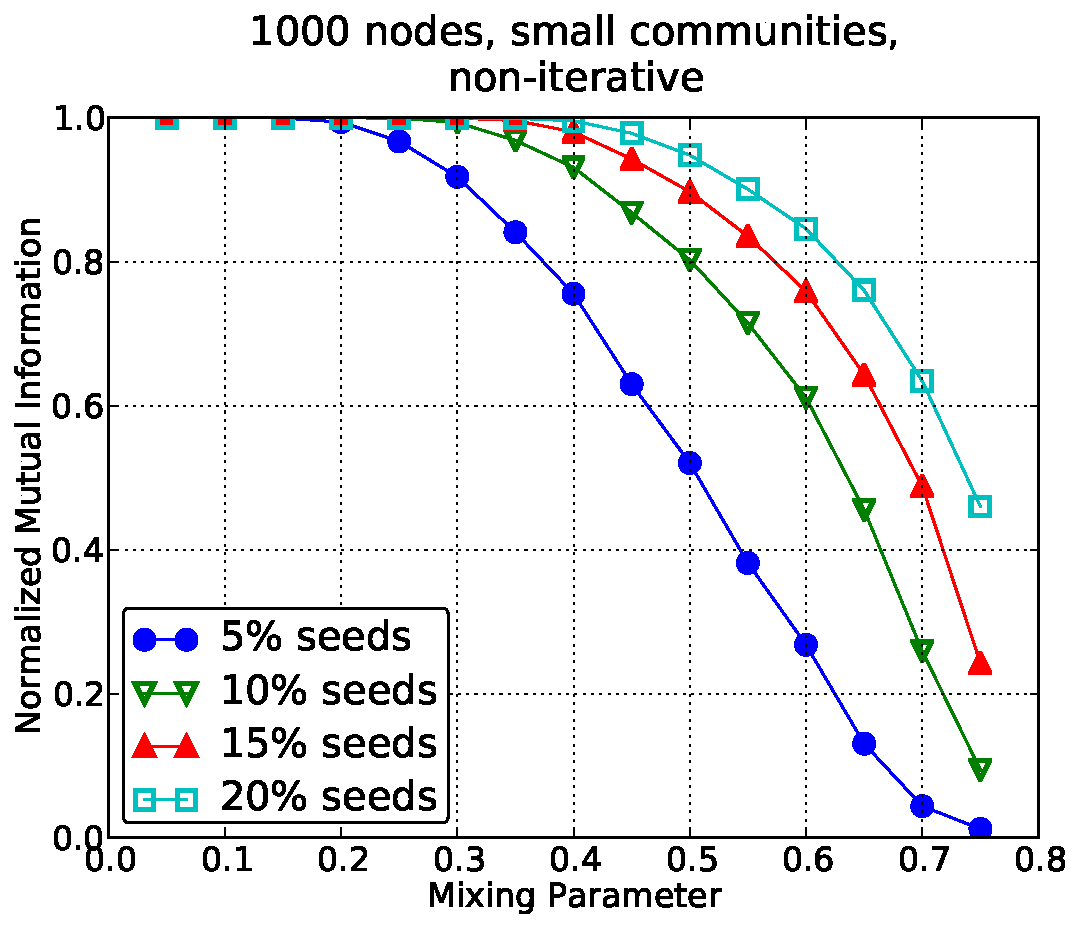
\includegraphics[width=\plotwidth]{plots/nonoverlap_noniter_a.pdf}
    \end{subfigure}%
    \begin{subfigure}{0.5\textwidth}
    \centering
    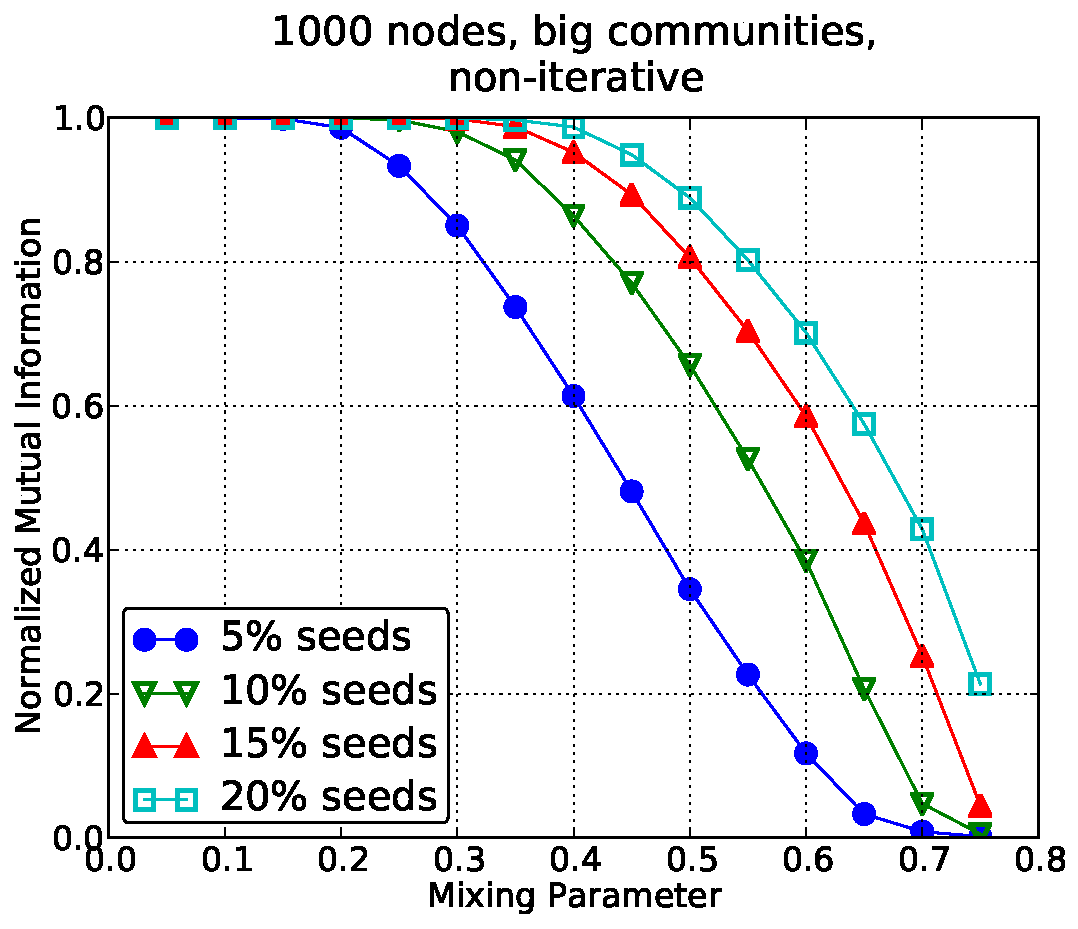
\includegraphics[width=\plotwidth]{plots/nonoverlap_noniter_b.pdf}
    \end{subfigure}
    \begin{subfigure}{0.5\textwidth}
    \centering
    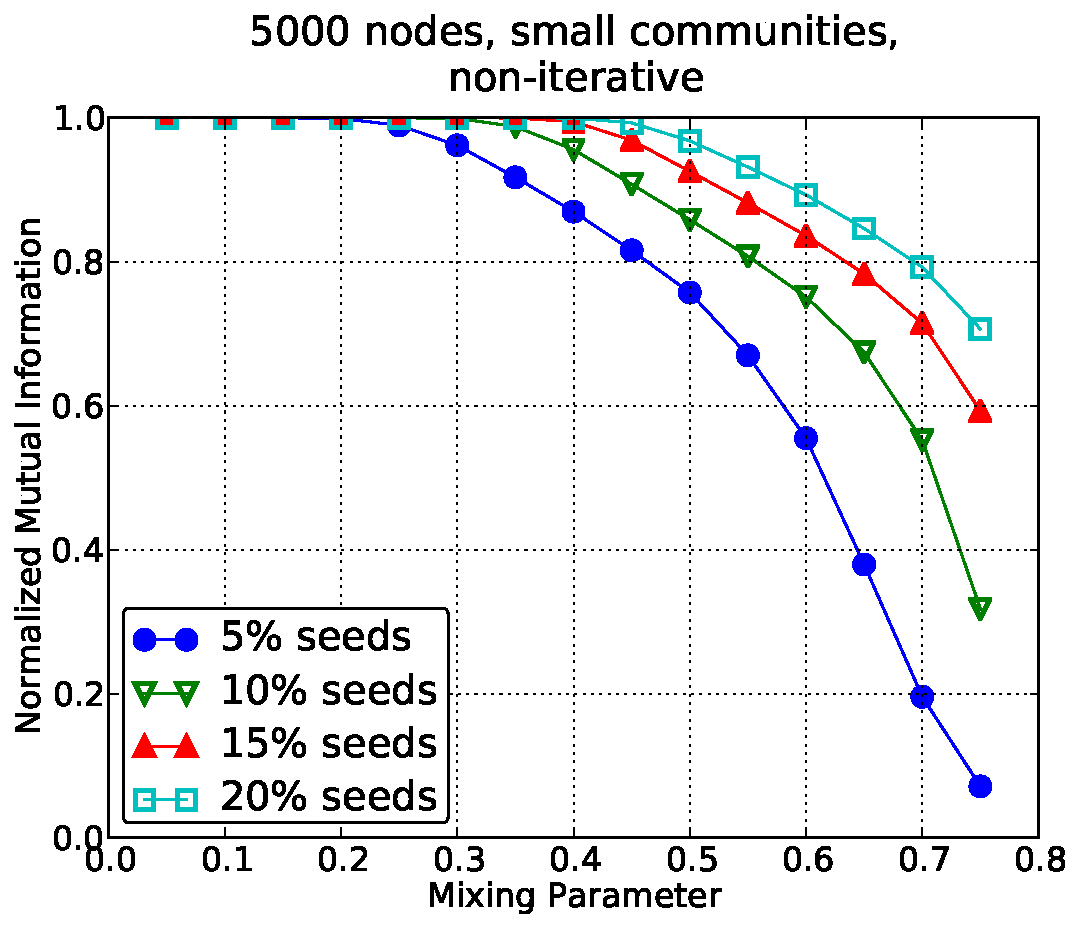
\includegraphics[width=\plotwidth]{plots/nonoverlap_noniter_c.pdf}
    \end{subfigure}%
    \begin{subfigure}{0.5\textwidth}
    \centering
    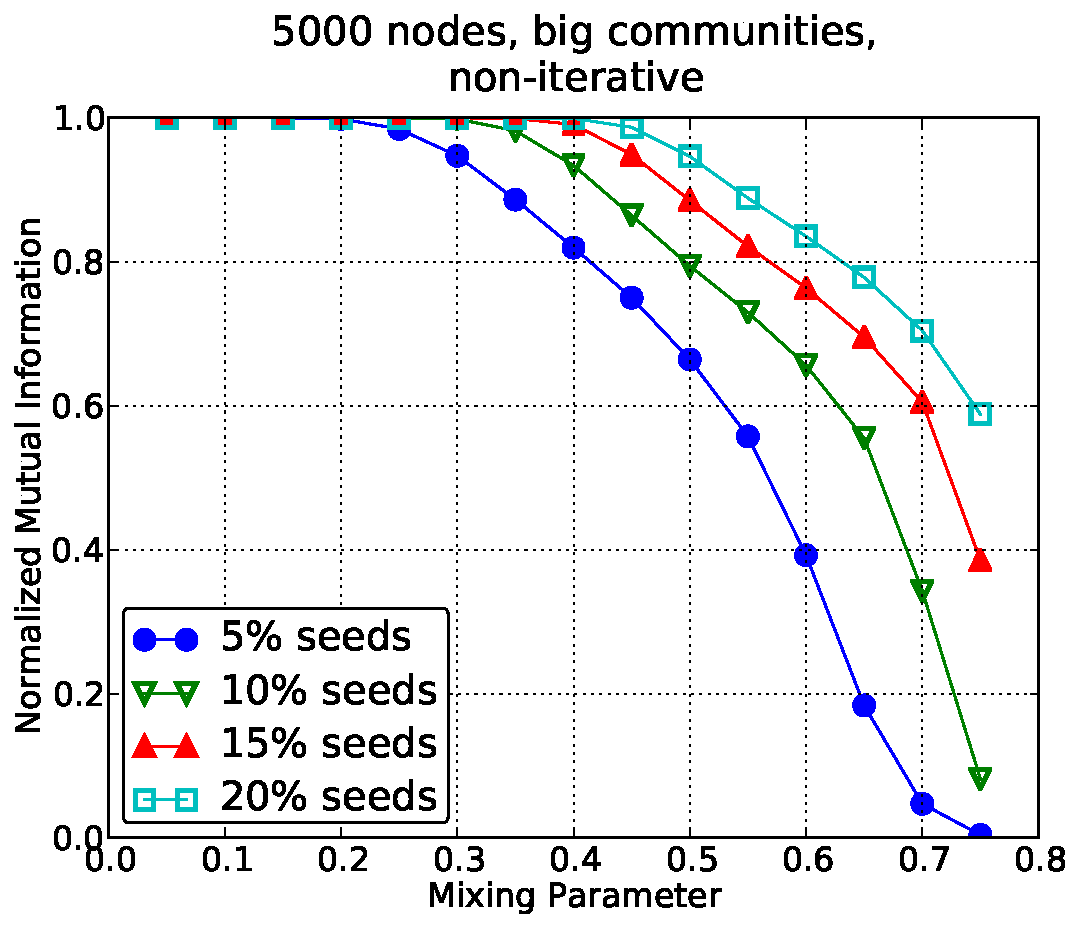
\includegraphics[width=\plotwidth]{plots/nonoverlap_noniter_d.pdf}
    \end{subfigure}
    \caption{Non-iterative method for non-overlapping communities.}\label{fig:no_iter_no_overlap}
%\end{figure}
%
%\begin{figure}[h!]
    \centering
    \begin{subfigure}{0.5\textwidth}
    \centering
    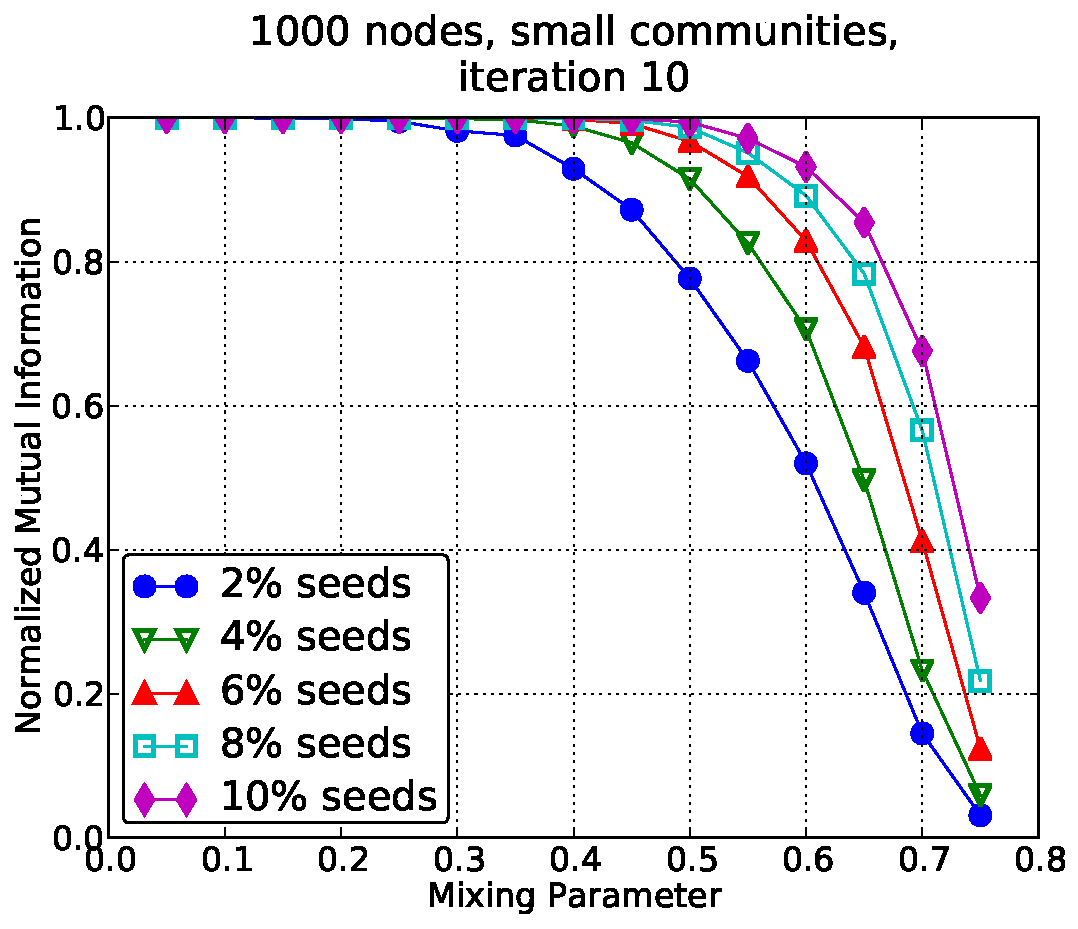
\includegraphics[width=\plotwidth]{plots/nonoverlap_iter_a.pdf}
    \end{subfigure}%
    \begin{subfigure}{0.5\textwidth}
    \centering
    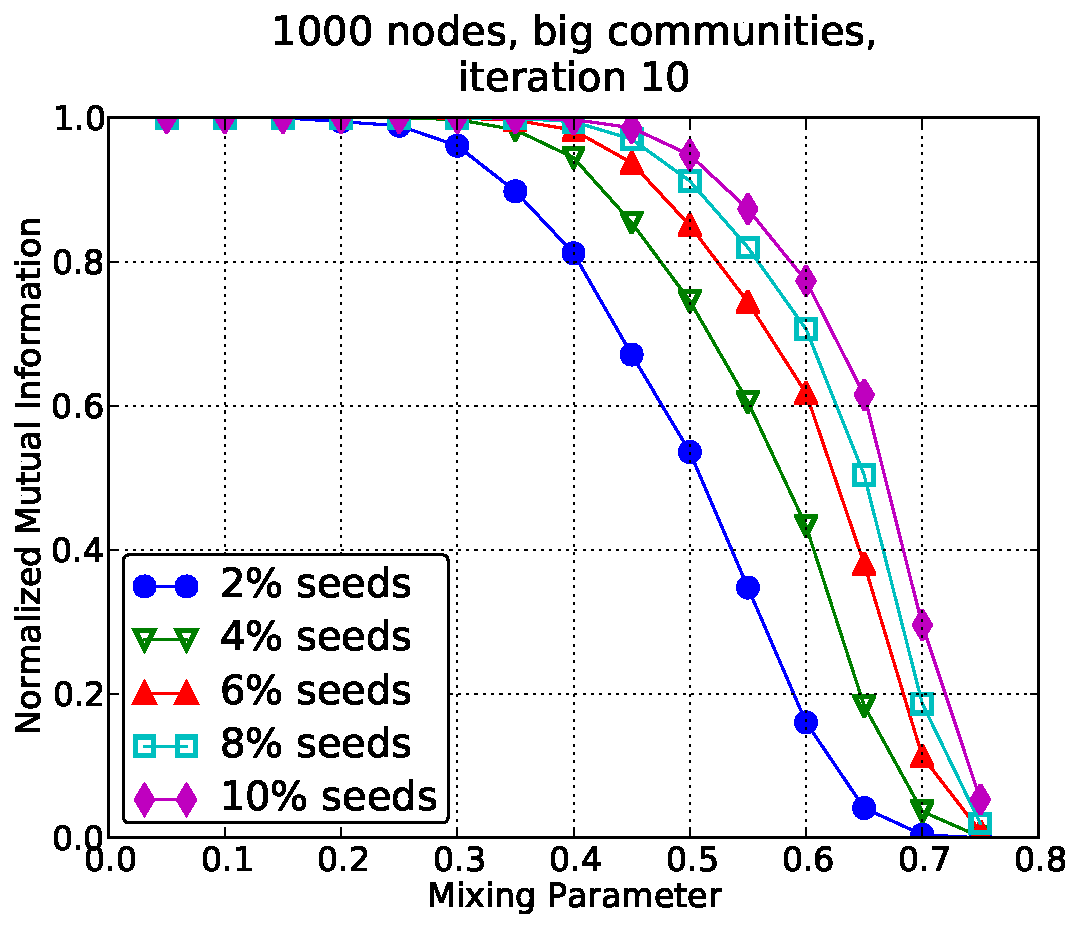
\includegraphics[width=\plotwidth]{plots/nonoverlap_iter_b.pdf}
    \end{subfigure}
    \begin{subfigure}{0.5\textwidth}
    \centering
    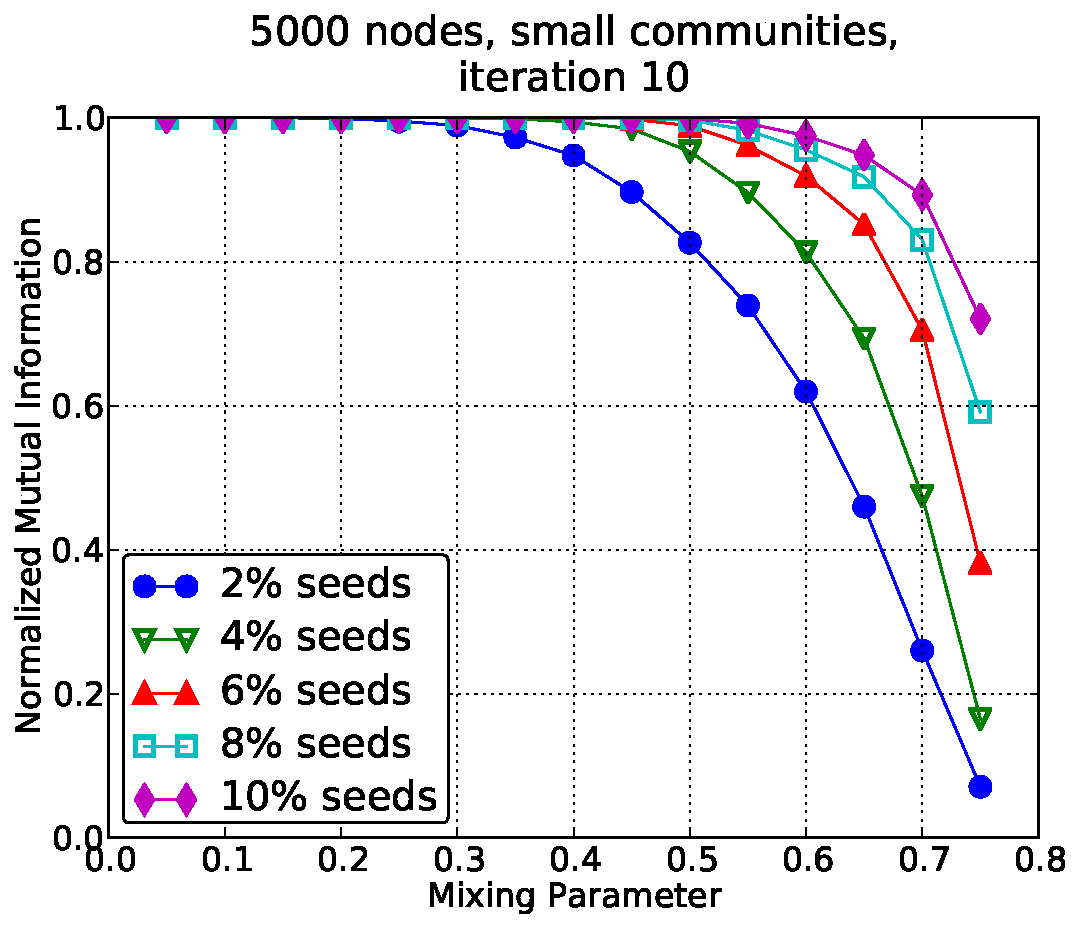
\includegraphics[width=\plotwidth]{plots/nonoverlap_iter_c.pdf}
    \end{subfigure}%
    \begin{subfigure}{0.5\textwidth}
    \centering
    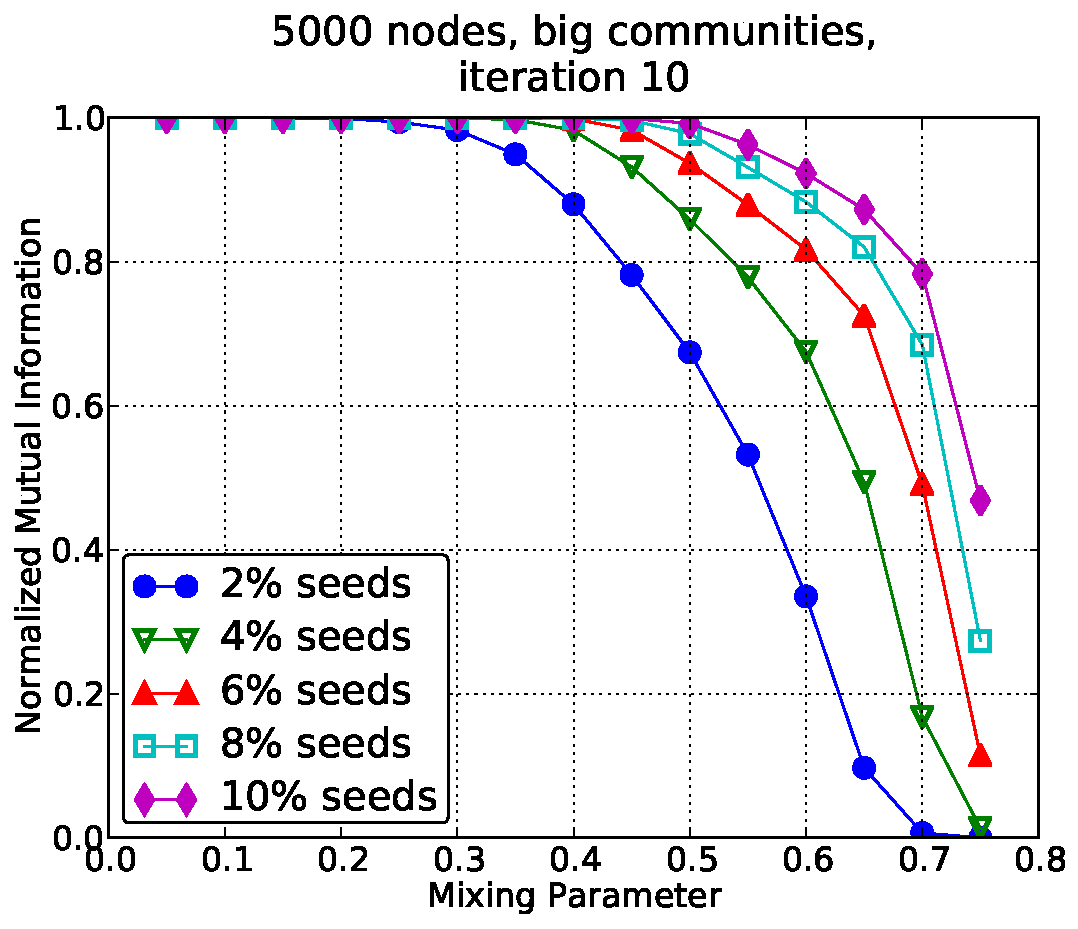
\includegraphics[width=\plotwidth]{plots/nonoverlap_iter_d.pdf}
    \end{subfigure}
    \caption{Iterative method for non-overlapping communities.}\label{fig:iter_no_overlap}
\end{figure}
%

%\begin{figure}[h!]
%    \centering
%    \begin{subfigure}{0.5\textwidth}
%    \centering
%    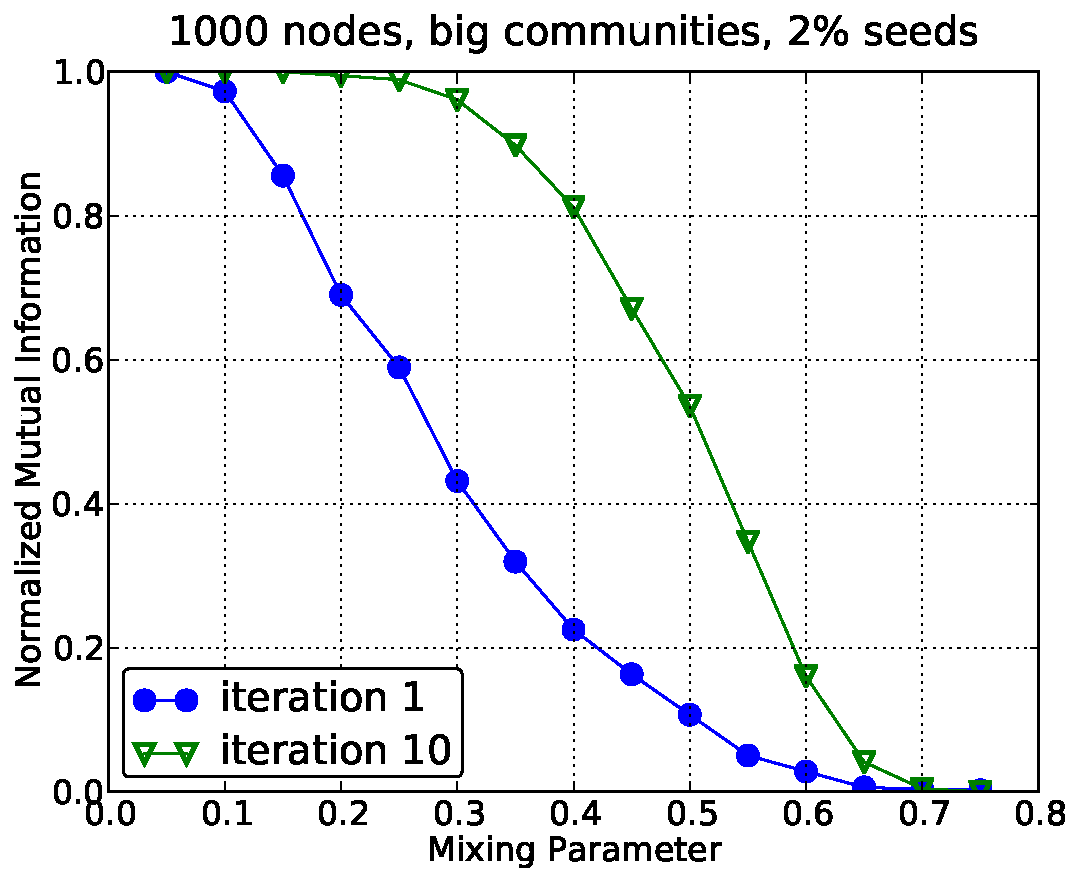
\includegraphics[width=\plotwidth]{plots/nonoverlap_compare_a.pdf}
%    \end{subfigure}%
%    \begin{subfigure}{0.5\textwidth}
%    \centering
%    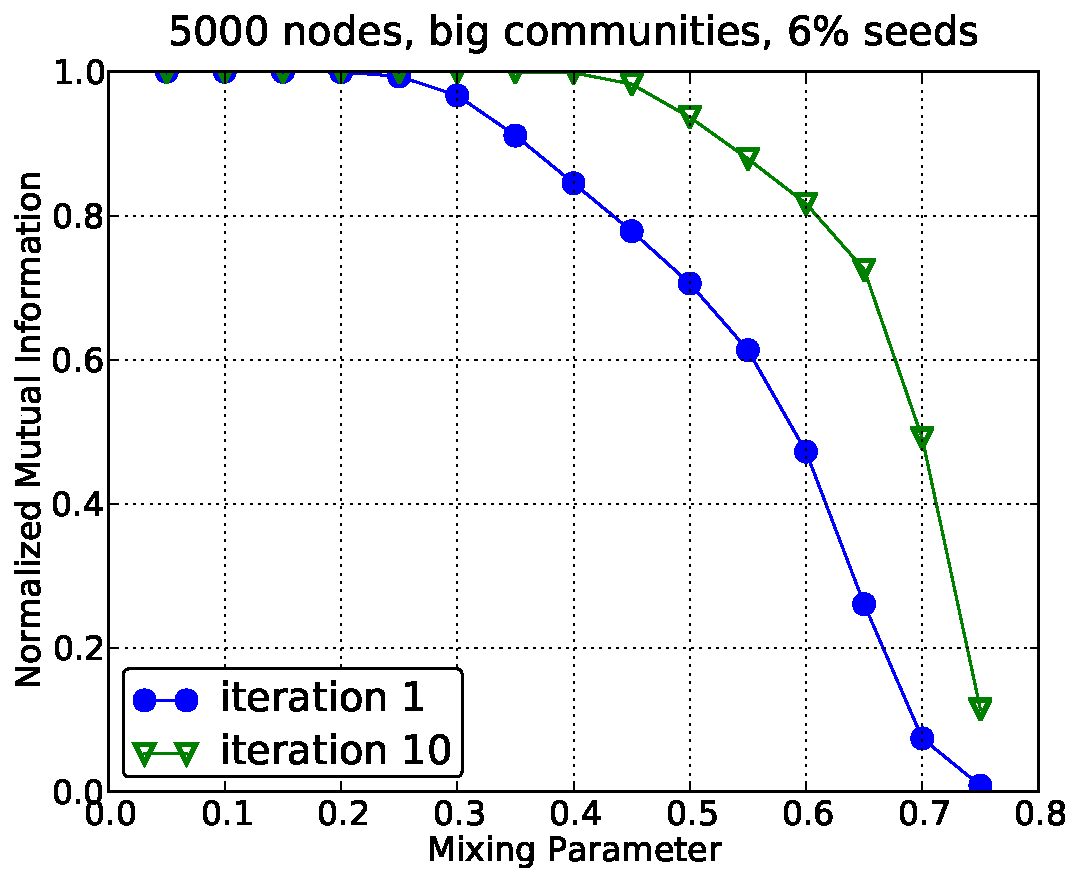
\includegraphics[width=\plotwidth]{plots/nonoverlap_compare_b.pdf}
%    \end{subfigure}
%    \caption{Comparison between the iterative and non-iterative method for 
%		non-overlapping communities.}\label{fig:compare_iter_no_overlap}
%\end{figure}

\begin{figure}[h!]
    \centering
    \begin{subfigure}{0.35\textwidth}
    \centering
    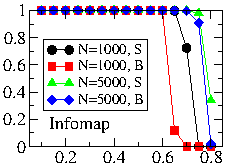
\includegraphics[width=\otherplotswidth]{lfrpaper/1_split_kropped.pdf}
    \end{subfigure}%
    \begin{subfigure}{0.35\textwidth}
    \centering
    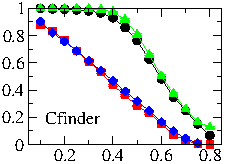
\includegraphics[width=\otherplotswidth]{lfrpaper/2_split_kropped.pdf}
    \end{subfigure}%
    \begin{subfigure}{0.35\textwidth}
    \centering
    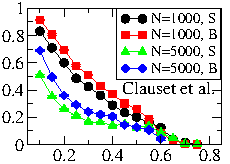
\includegraphics[width=\otherplotswidth]{lfrpaper/3_split_kropped.pdf}
    \end{subfigure}
    \begin{subfigure}{0.35\textwidth}
    \centering
    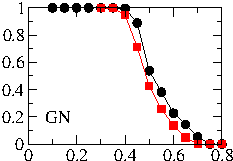
\includegraphics[width=\otherplotswidth]{lfrpaper/4_split_kropped.pdf}
    \end{subfigure}%
    \begin{subfigure}{0.35\textwidth}
    \centering
    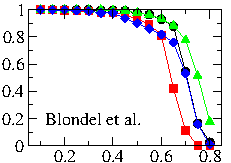
\includegraphics[width=\otherplotswidth]{lfrpaper/5_split_kropped.pdf}
    \end{subfigure}%
    \begin{subfigure}{0.35\textwidth}
    \centering
    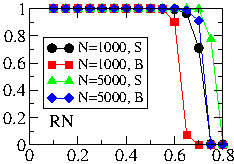
\includegraphics[width=\otherplotswidth]{lfrpaper/6_split_kropped.pdf}
    \end{subfigure}%
    \caption{
        Plots for Infomap, CFinder, the algorithm of Clauset \etal, Girvan-Newman (GN), Blondel \etal, 
        and the Pott's model approach by Ronhovde and Nussinov (RN) on the LFR benchmark for non-overlapping 
		communities. As usual, the NMI-value ($y$-axis) is plotted against the mixing factor ($x$-axis).
        Tests were performed on graphs with 1000 and 5000 nodes with big (B) and small (S) communities.
        Reproduced from~\cite{LF09}.
    }\label{fig:Infomap_etal}
\end{figure}

\begin{figure}[h!]
    \centering
    \begin{subfigure}{0.5\textwidth}
    \centering
    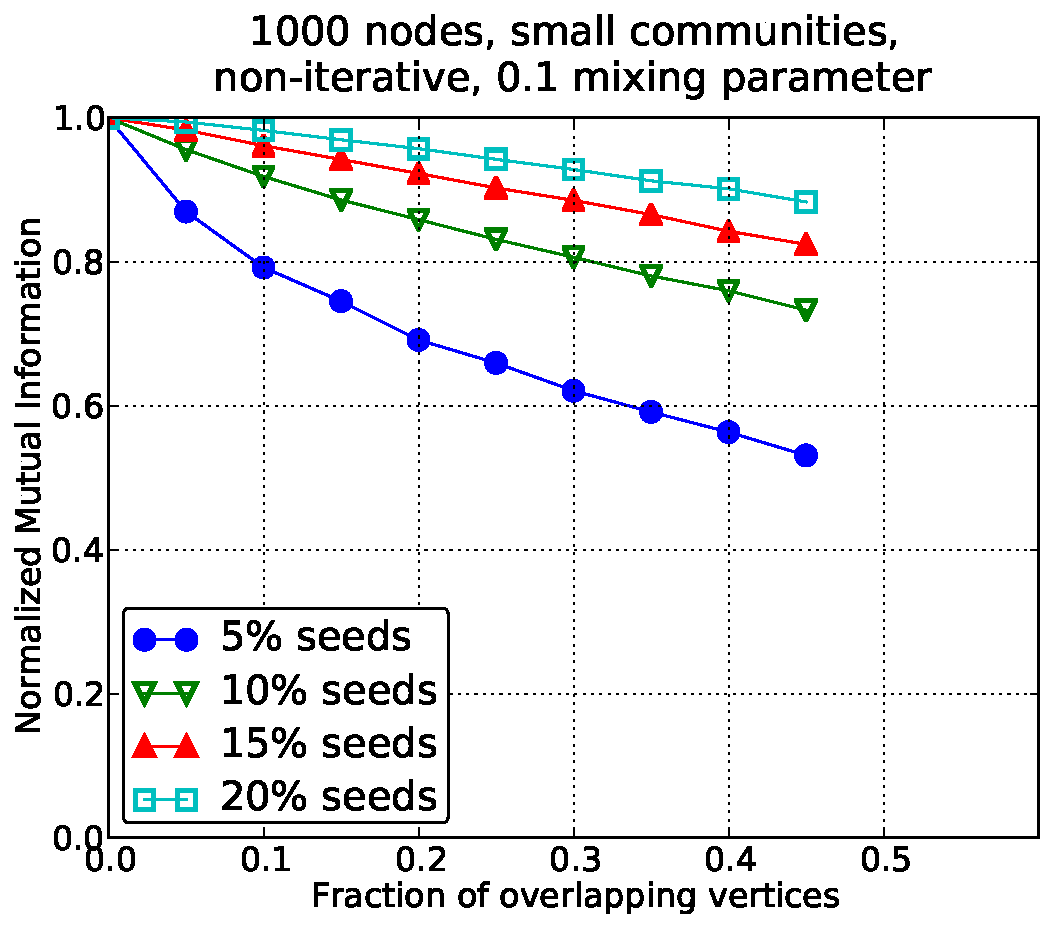
\includegraphics[width=\plotwidth]{plots/overlap_noniter_1mu_a.pdf}
    \end{subfigure}%
    \begin{subfigure}{0.5\textwidth}
    \centering
    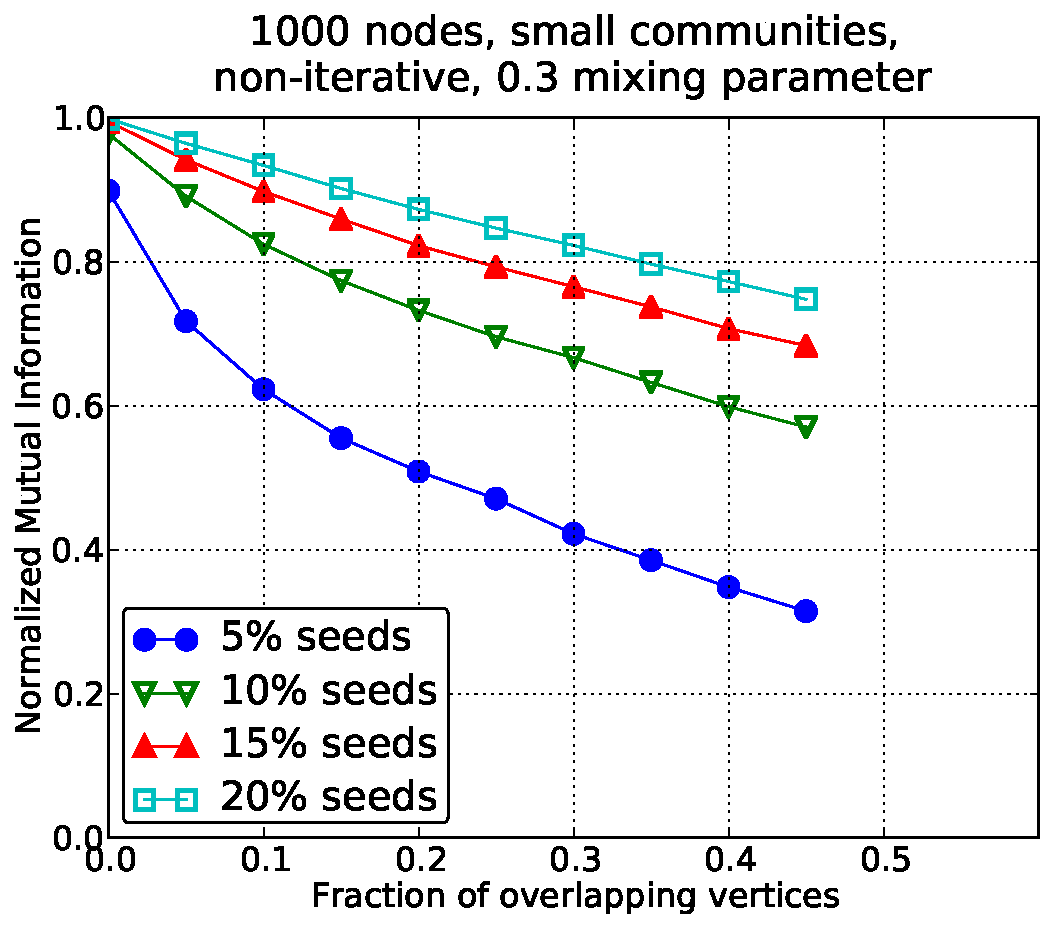
\includegraphics[width=\plotwidth]{plots/overlap_noniter_3mu_a.pdf}
    \end{subfigure}
    \begin{subfigure}{0.5\textwidth}
    \centering
    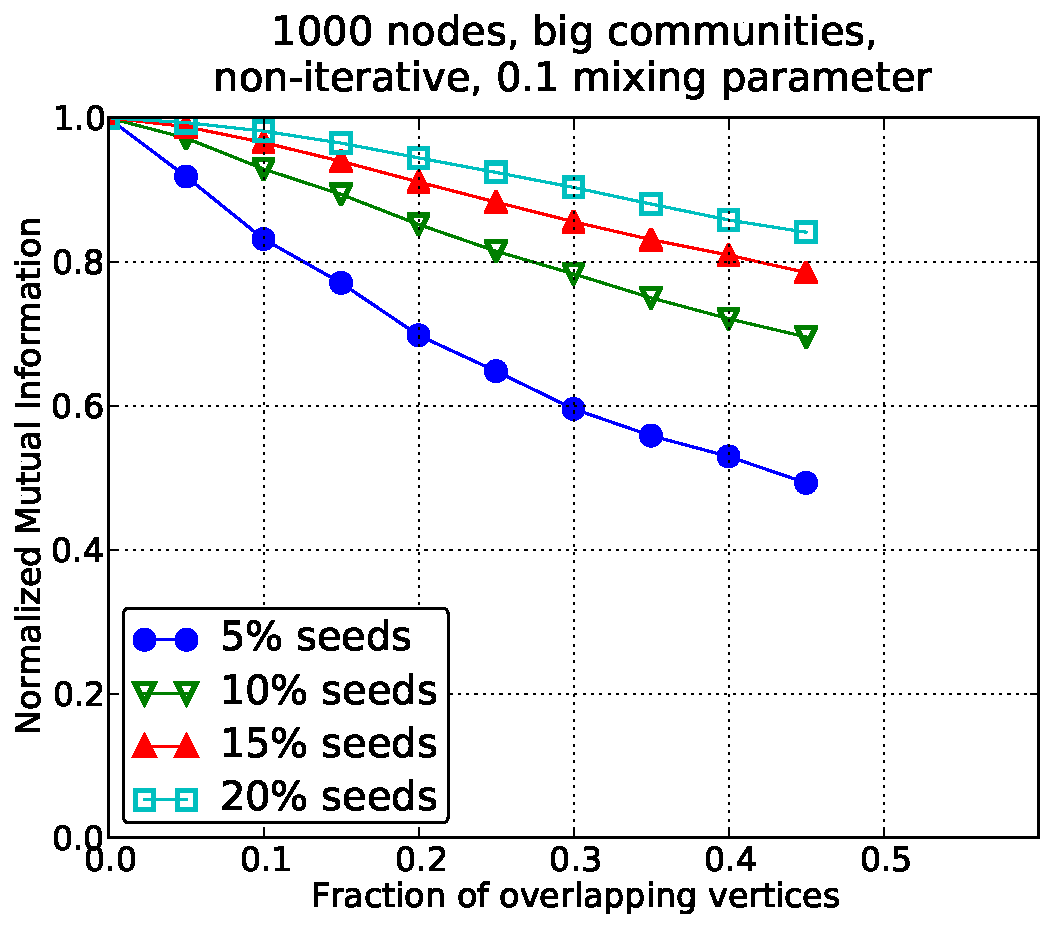
\includegraphics[width=\plotwidth]{plots/overlap_noniter_1mu_b.pdf}
    \end{subfigure}%
    \begin{subfigure}{0.5\textwidth}
    \centering
    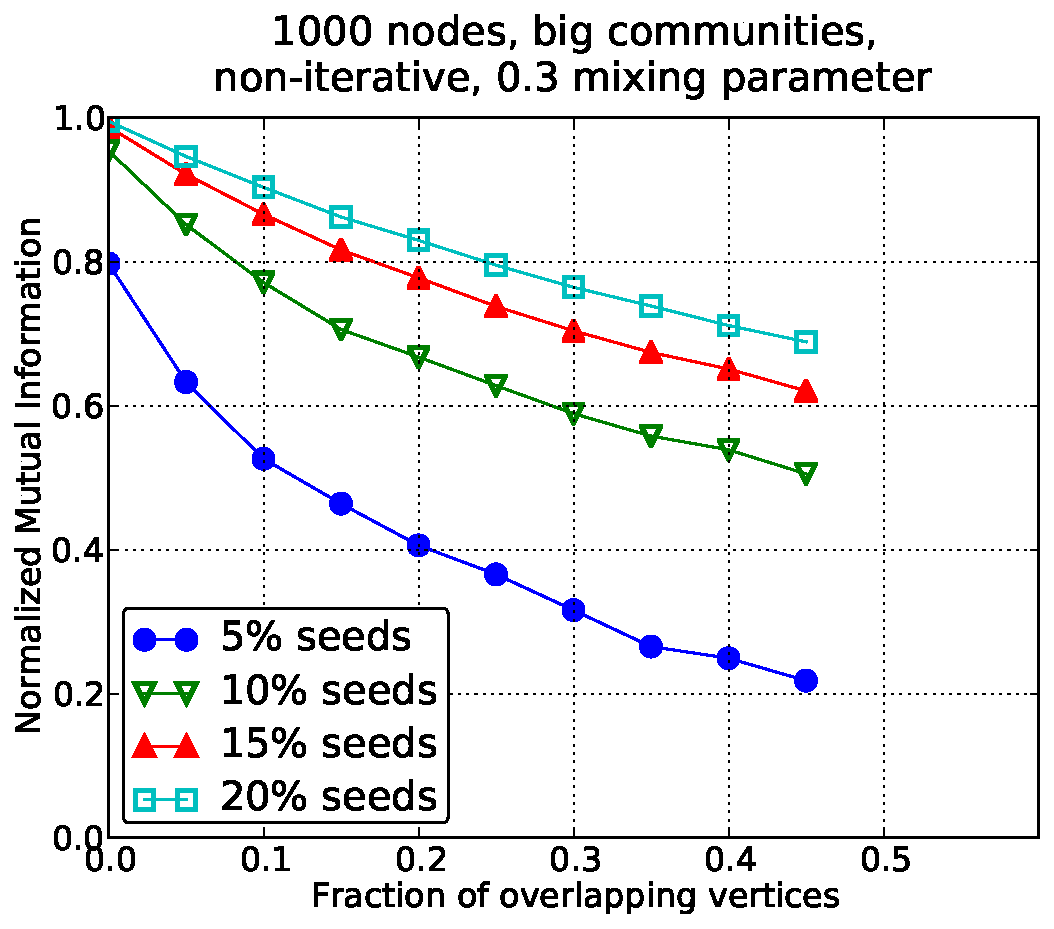
\includegraphics[width=\plotwidth]{plots/overlap_noniter_3mu_b.pdf}
    \end{subfigure}
    \caption{Non-iterative method for overlapping communities on 1000 nodes.}\label{fig:no_iter_overlap_1000N}
%\end{figure}
%
%\begin{figure}[h!]
    \centering
    \begin{subfigure}{0.5\textwidth}
    \centering
    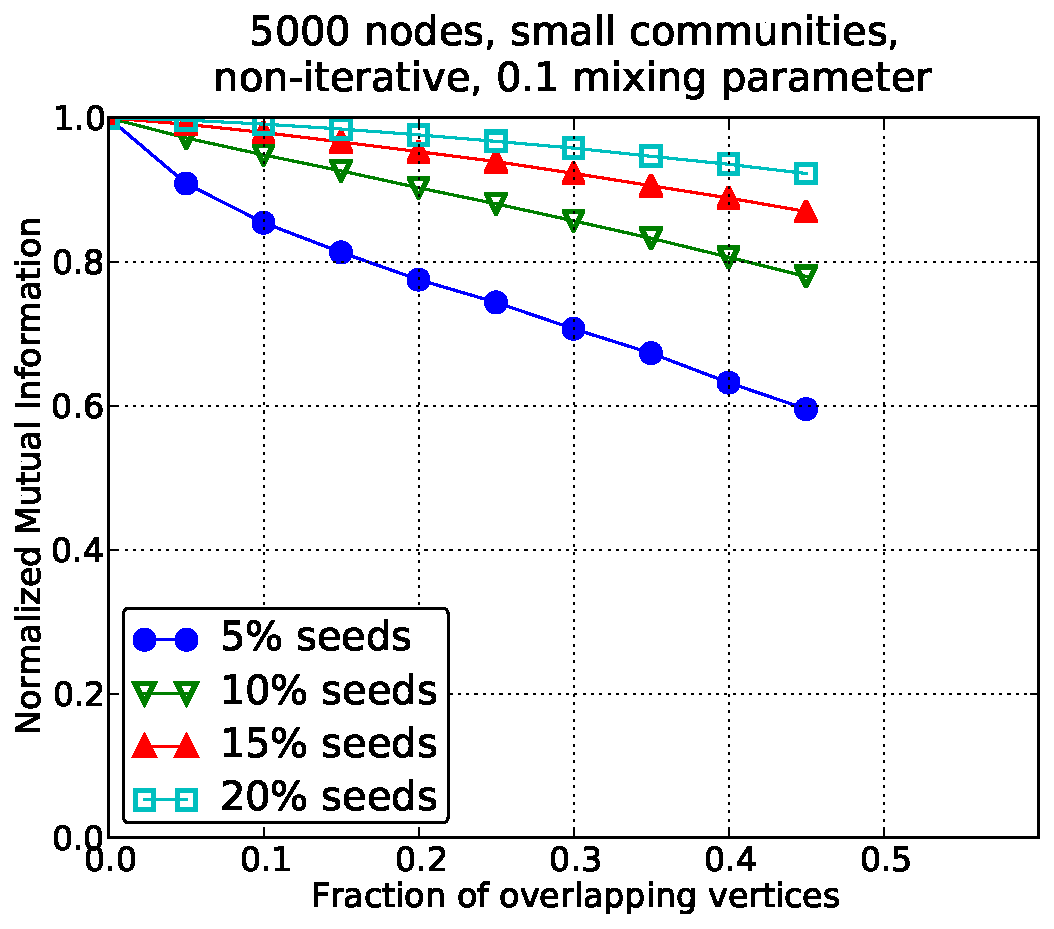
\includegraphics[width=\plotwidth]{plots/overlap_noniter_1mu_c.pdf}
    \end{subfigure}%
    \begin{subfigure}{0.5\textwidth}
    \centering
    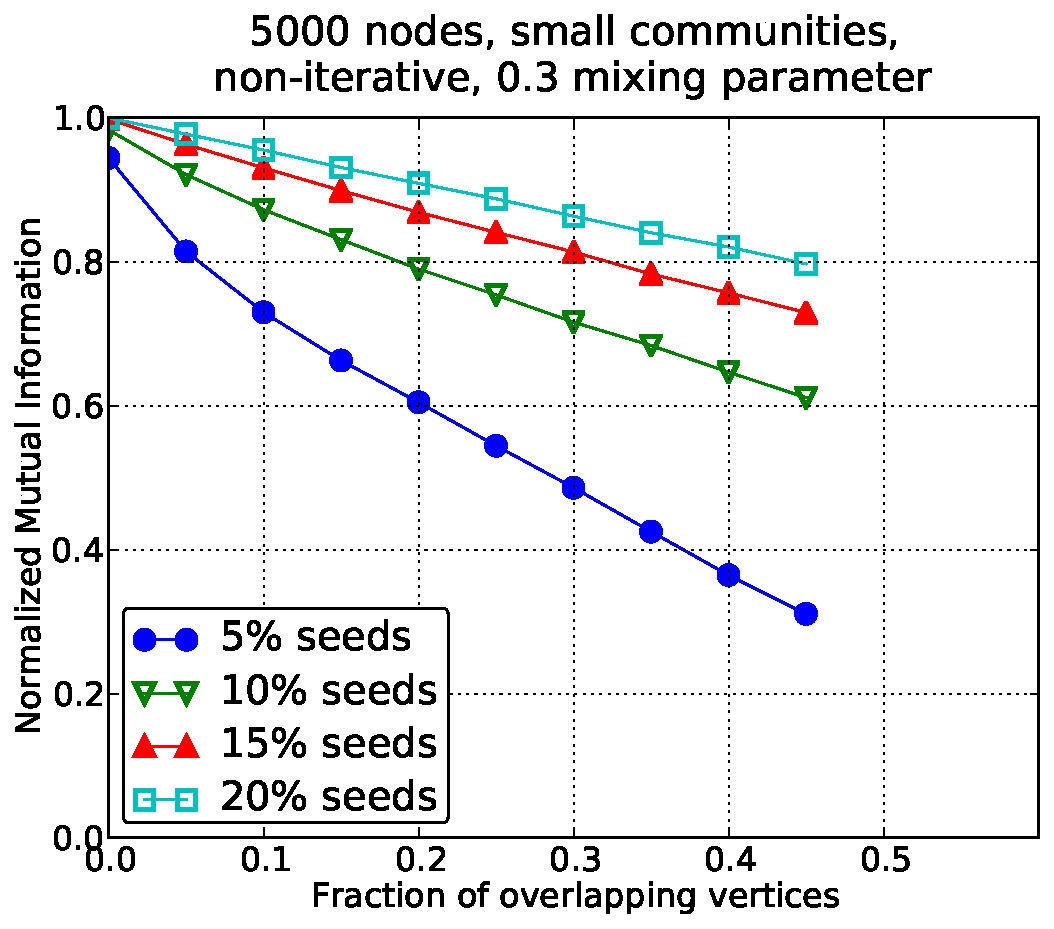
\includegraphics[width=\plotwidth]{plots/overlap_noniter_3mu_c.pdf}
    \end{subfigure}
    \begin{subfigure}{0.5\textwidth}
    \centering
    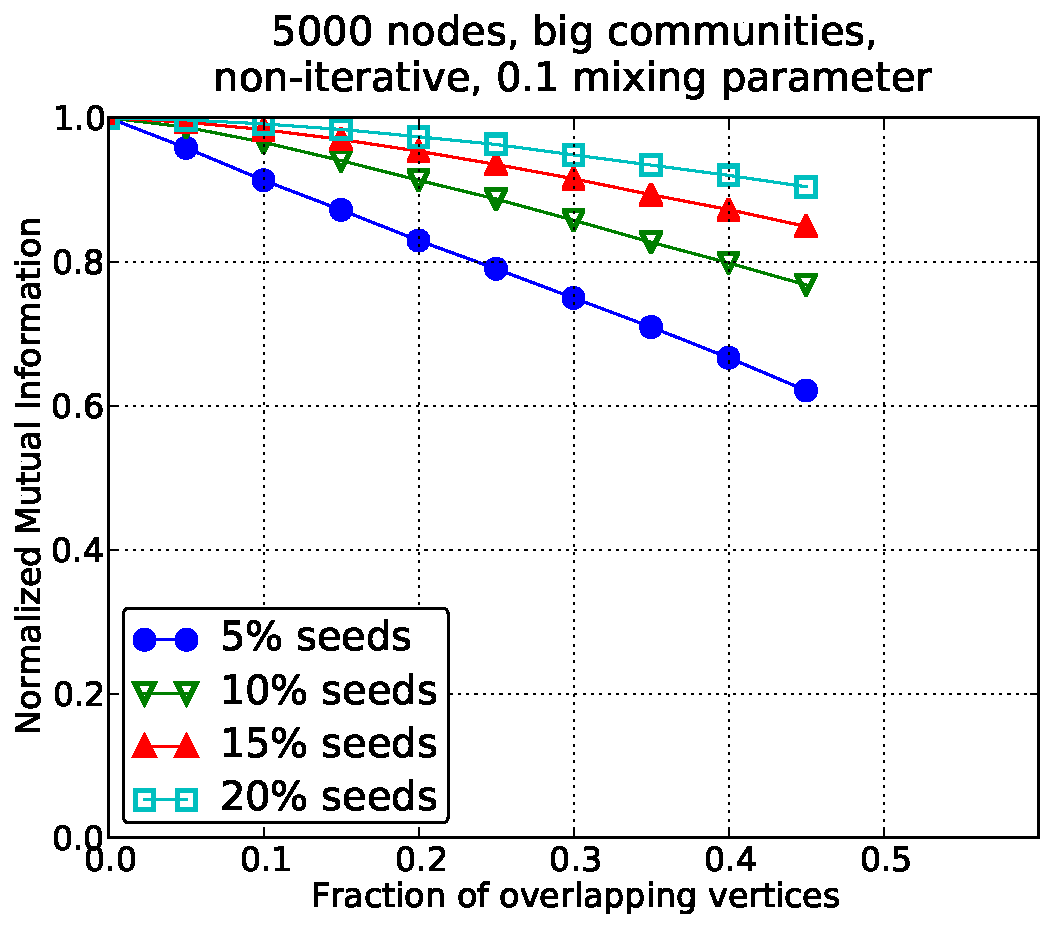
\includegraphics[width=\plotwidth]{plots/overlap_noniter_1mu_d.pdf}
    \end{subfigure}%
    \begin{subfigure}{0.5\textwidth}
    \centering
    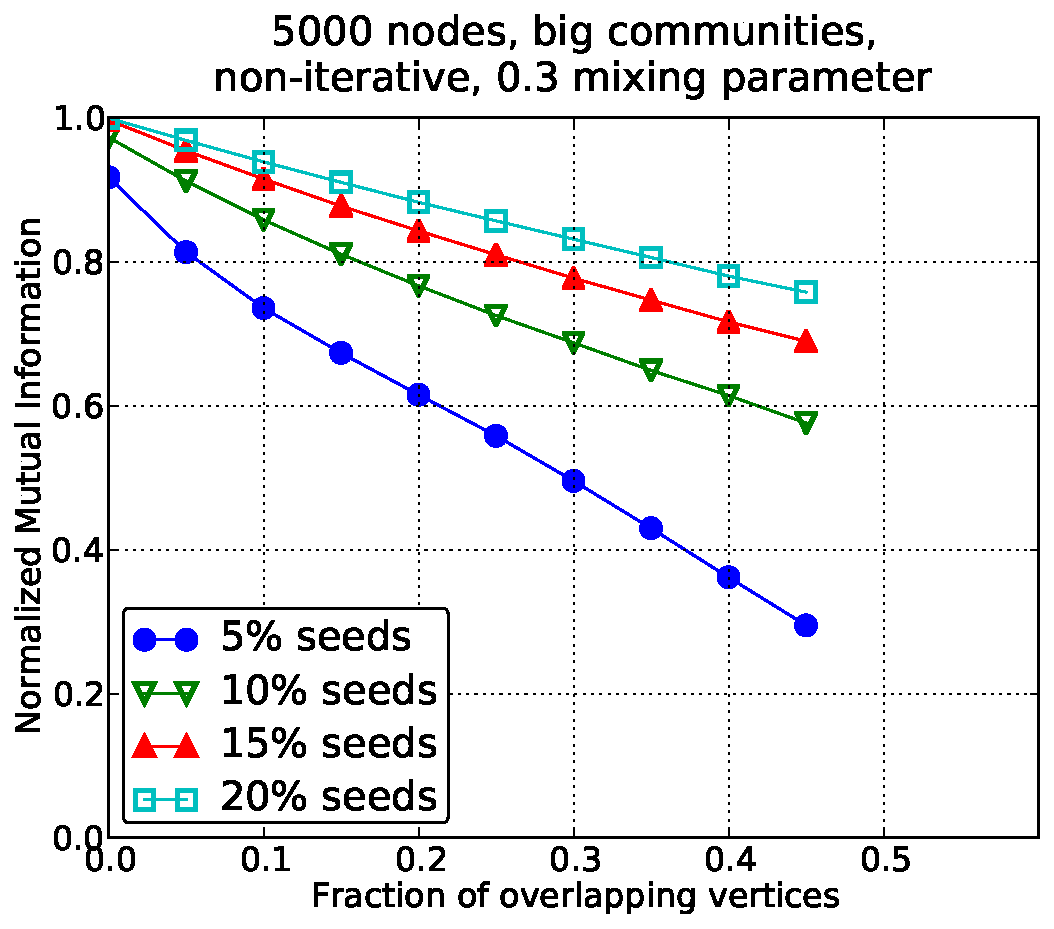
\includegraphics[width=\plotwidth]{plots/overlap_noniter_3mu_d.pdf}
    \end{subfigure}
    \caption{Non-iterative method for overlapping communities on 5000 nodes.}\label{fig:no_iter_overlap_5000N}
\end{figure}
%
\begin{figure}[h!]
    \centering
    \begin{subfigure}{0.5\textwidth}
    \centering
    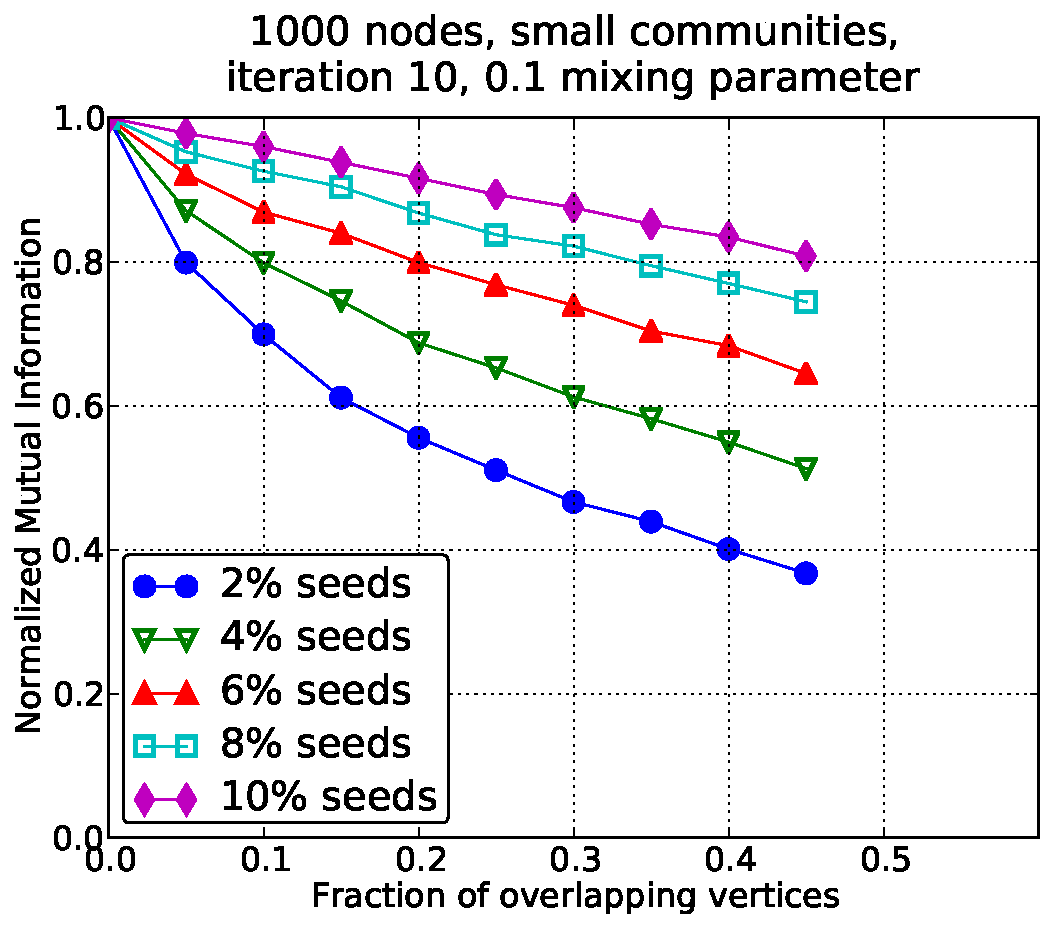
\includegraphics[width=\plotwidth]{plots/overlap_iter_1mu_a.pdf}
    \end{subfigure}%
    \begin{subfigure}{0.5\textwidth}
    \centering
    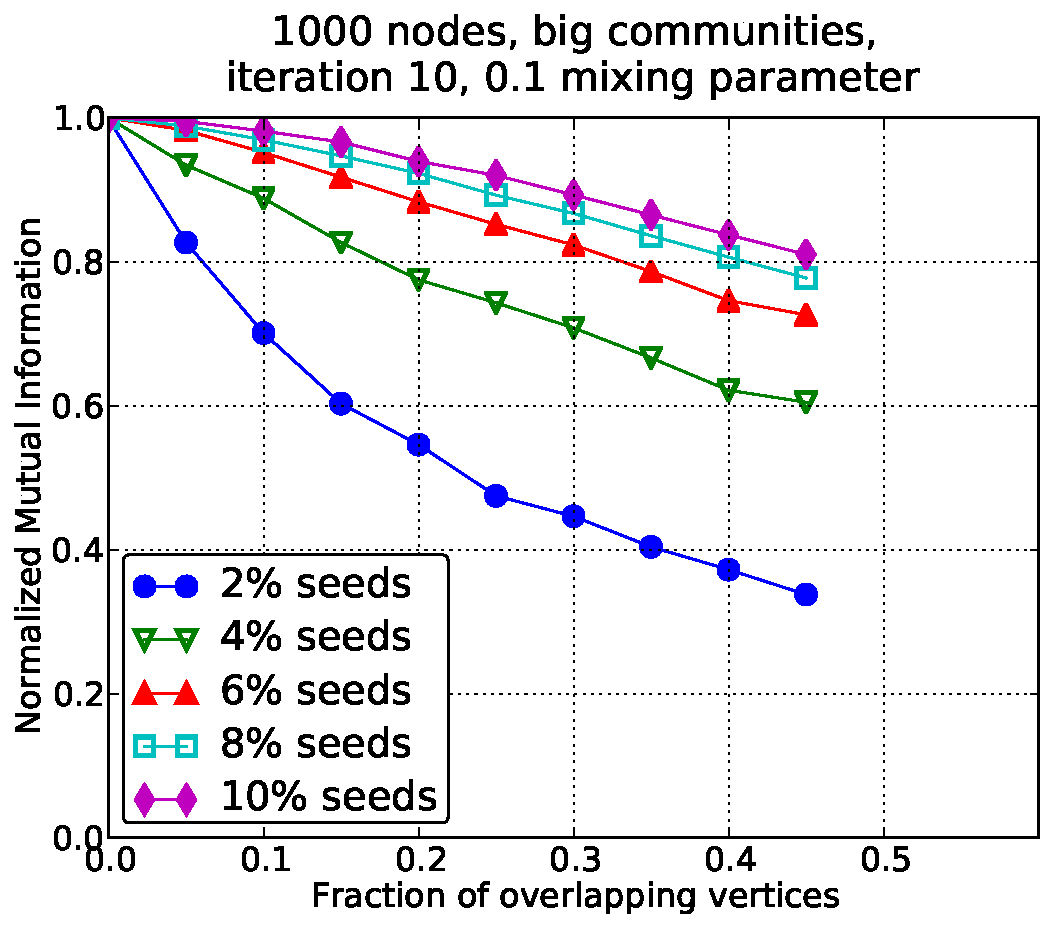
\includegraphics[width=\plotwidth]{plots/overlap_iter_1mu_b.pdf}
    \end{subfigure}
    \begin{subfigure}{0.5\textwidth}
    \centering
    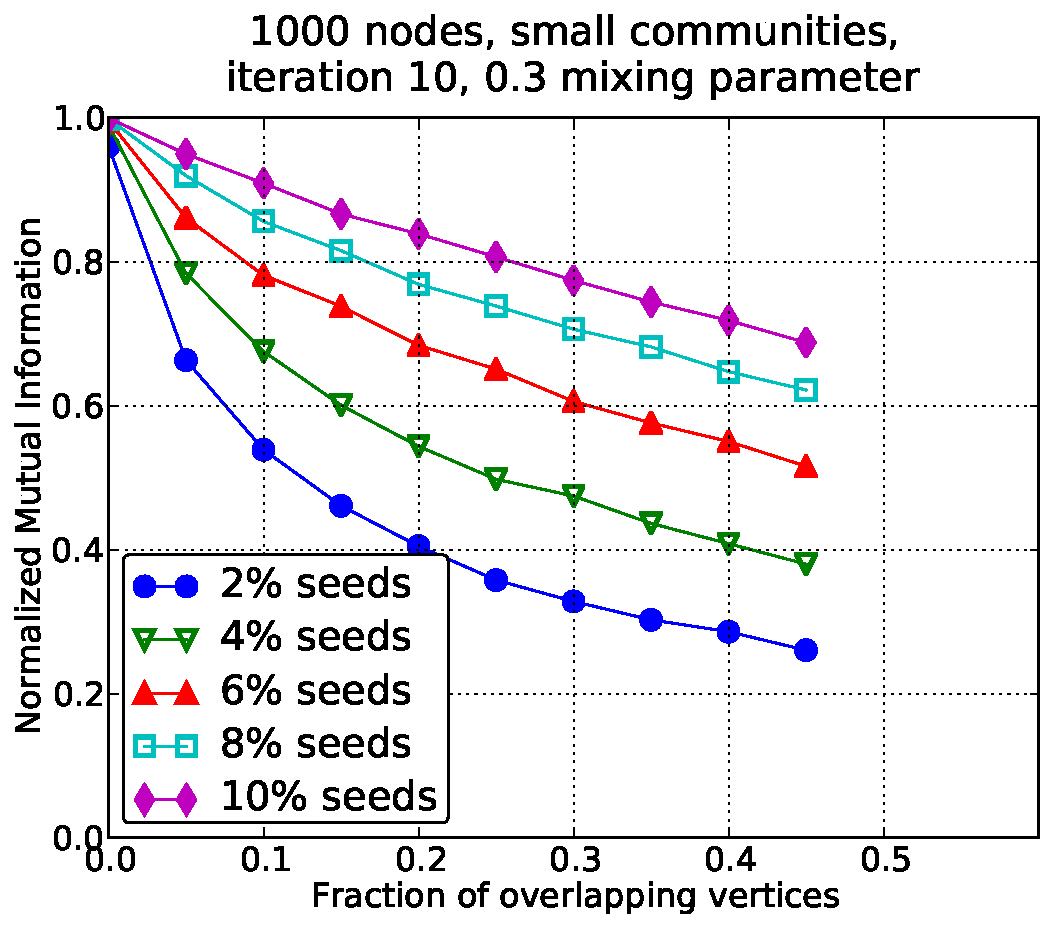
\includegraphics[width=\plotwidth]{plots/overlap_iter_3mu_a.pdf}
    \end{subfigure}%
    \begin{subfigure}{0.5\textwidth}
    \centering
    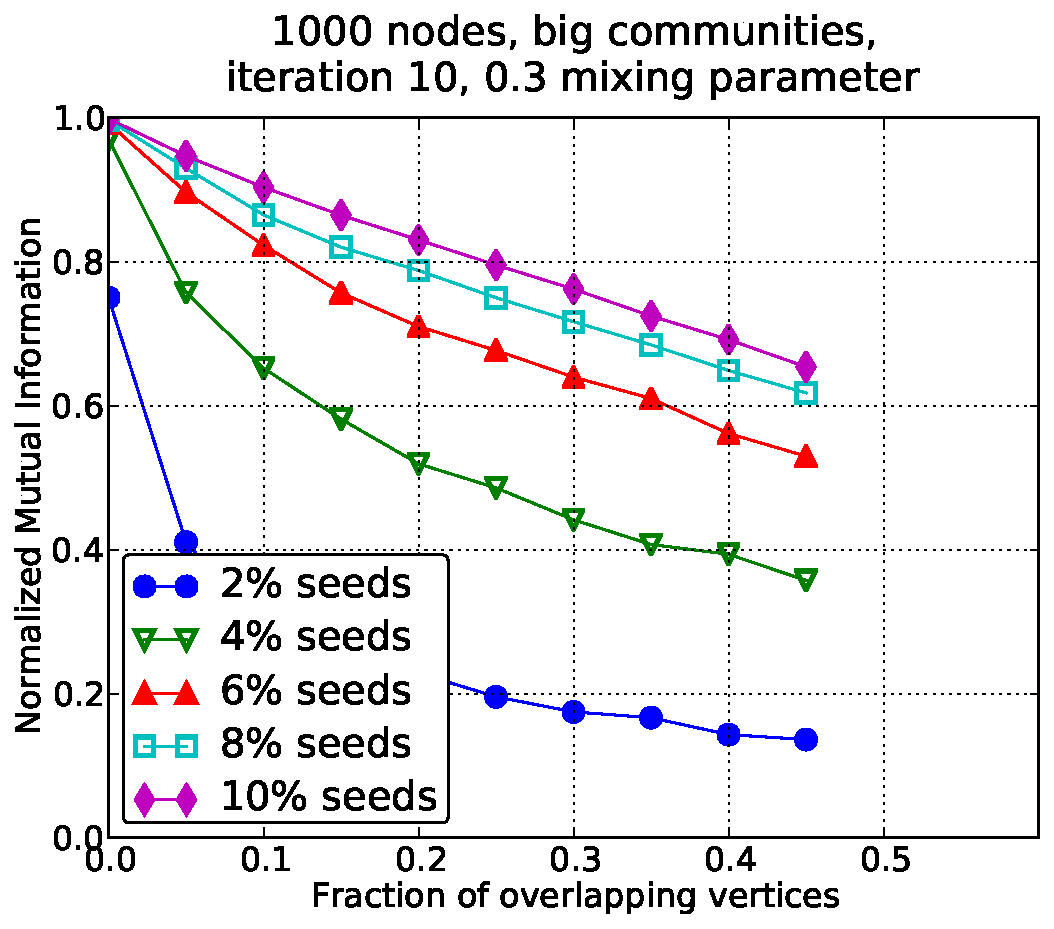
\includegraphics[width=\plotwidth]{plots/overlap_iter_3mu_b.pdf}
    \end{subfigure}
    \caption{Iterative method for overlapping communities on 1000 nodes.}\label{fig:iter_overlap_1000N}
%\end{figure}
%
%\begin{figure}[h!]
    \centering
    \begin{subfigure}{0.5\textwidth}
    \centering
    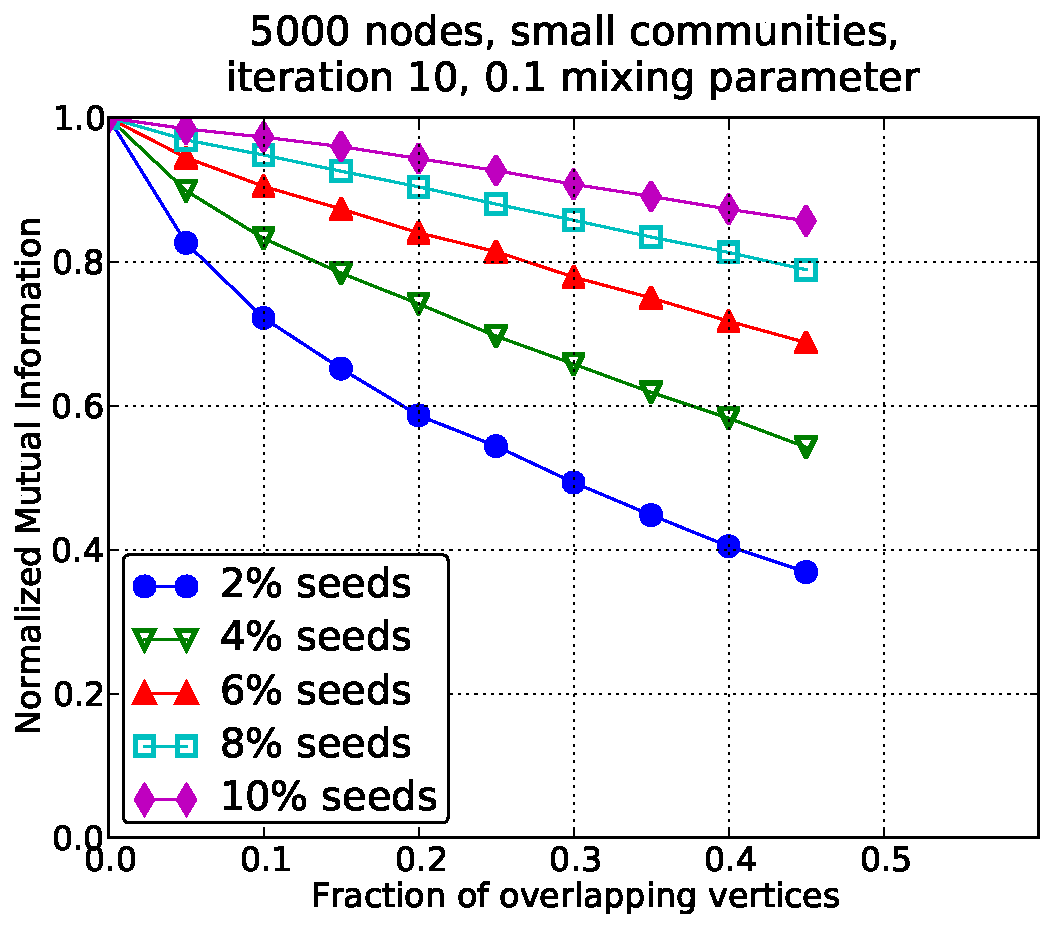
\includegraphics[width=\plotwidth]{plots/overlap_iter_1mu_c.pdf}
    \end{subfigure}%
    \begin{subfigure}{0.5\textwidth}
    \centering
    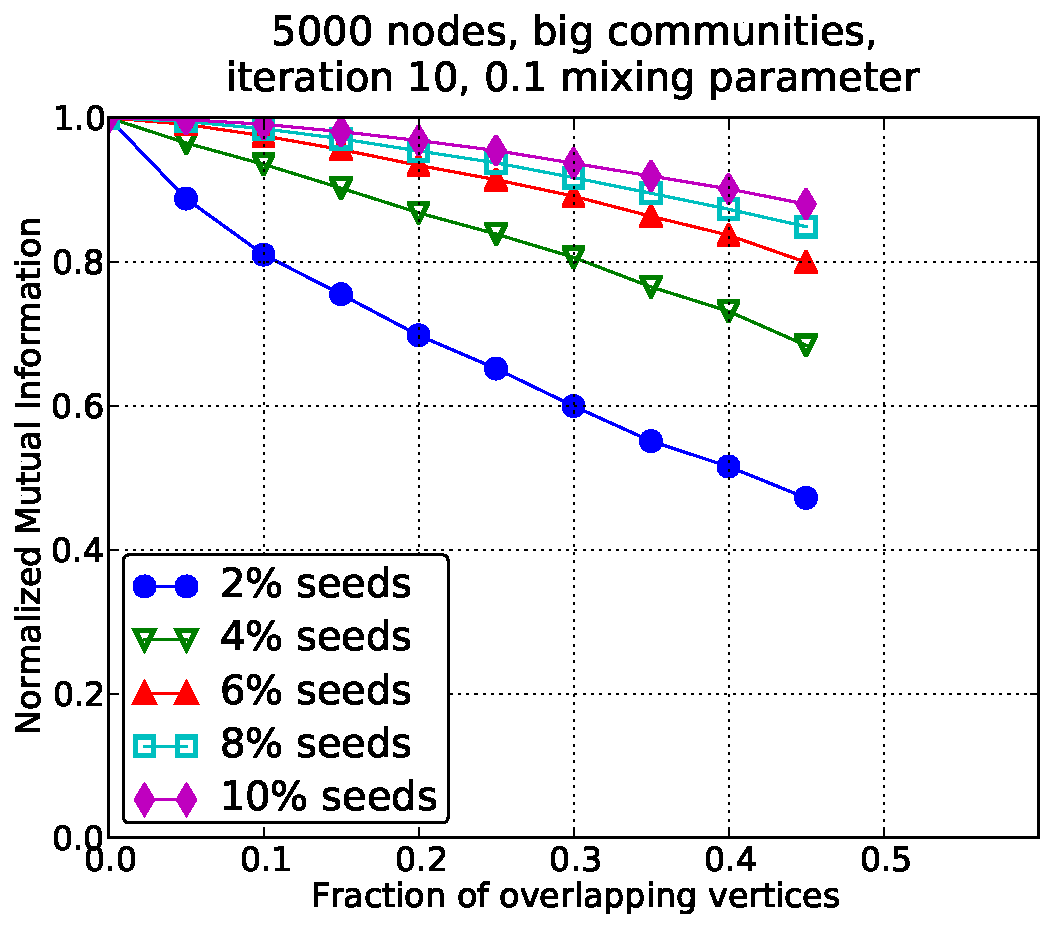
\includegraphics[width=\plotwidth]{plots/overlap_iter_1mu_d.pdf}
    \end{subfigure}
    \begin{subfigure}{0.5\textwidth}
    \centering
    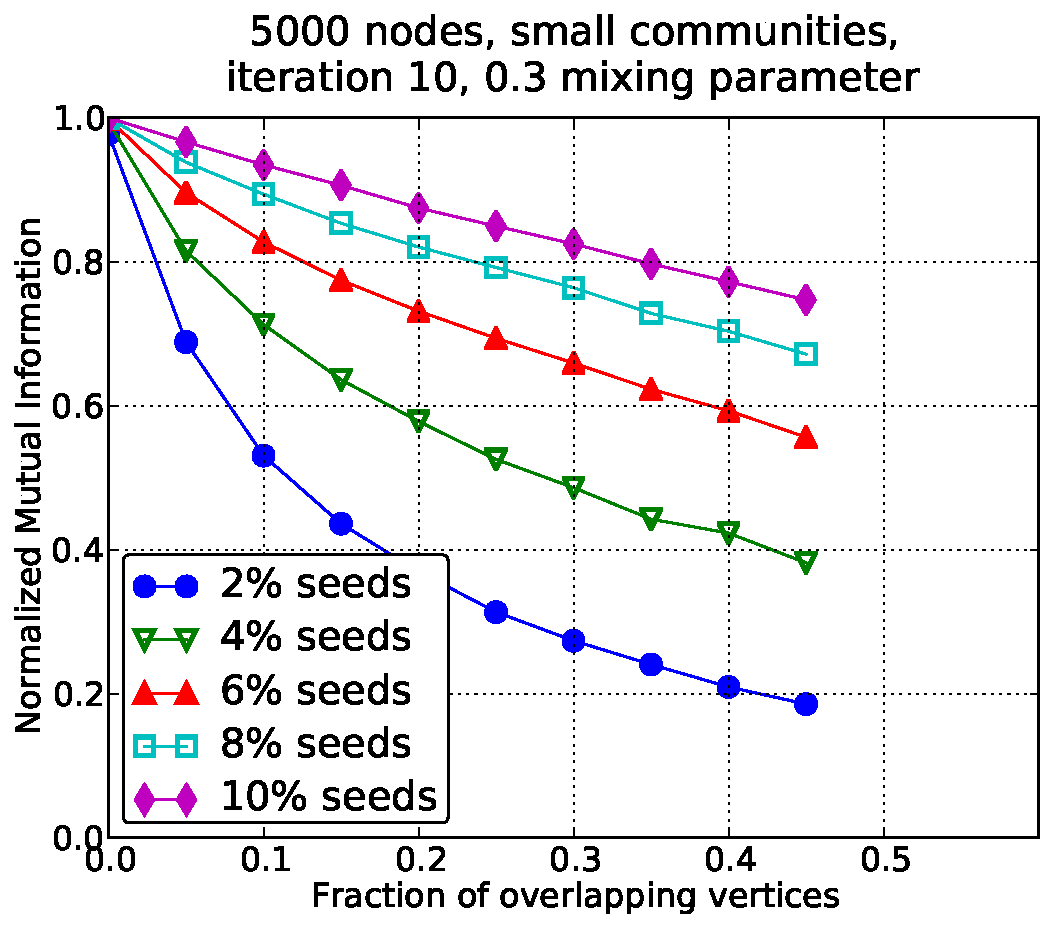
\includegraphics[width=\plotwidth]{plots/overlap_iter_3mu_c.pdf}
    \end{subfigure}%
    \begin{subfigure}{0.5\textwidth}
    \centering
    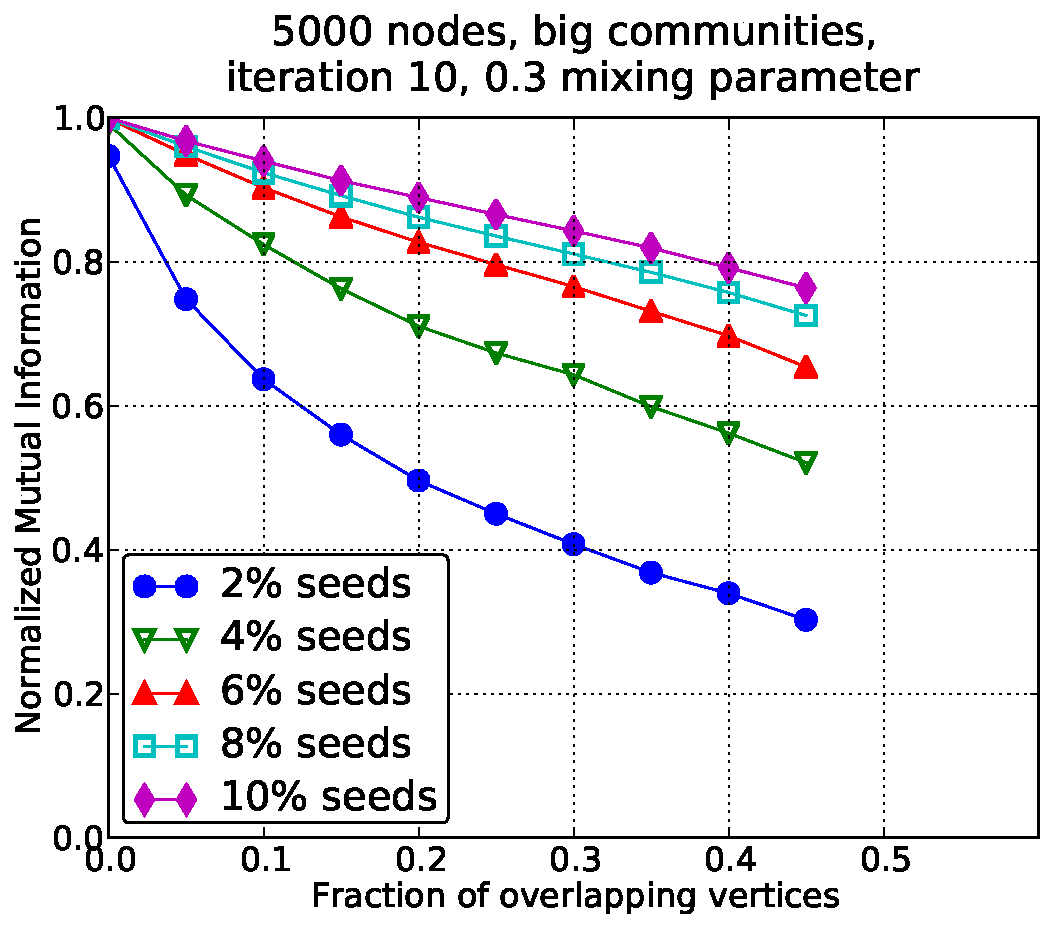
\includegraphics[width=\plotwidth]{plots/overlap_iter_3mu_d.pdf}
    \end{subfigure}
    \caption{Iterative method for overlapping communities on 5000 nodes.}\label{fig:iter_overlap_5000N}
\end{figure}
%
%\begin{figure}[h!]
%    \centering
%    \begin{subfigure}{0.5\textwidth}
%    \centering
%    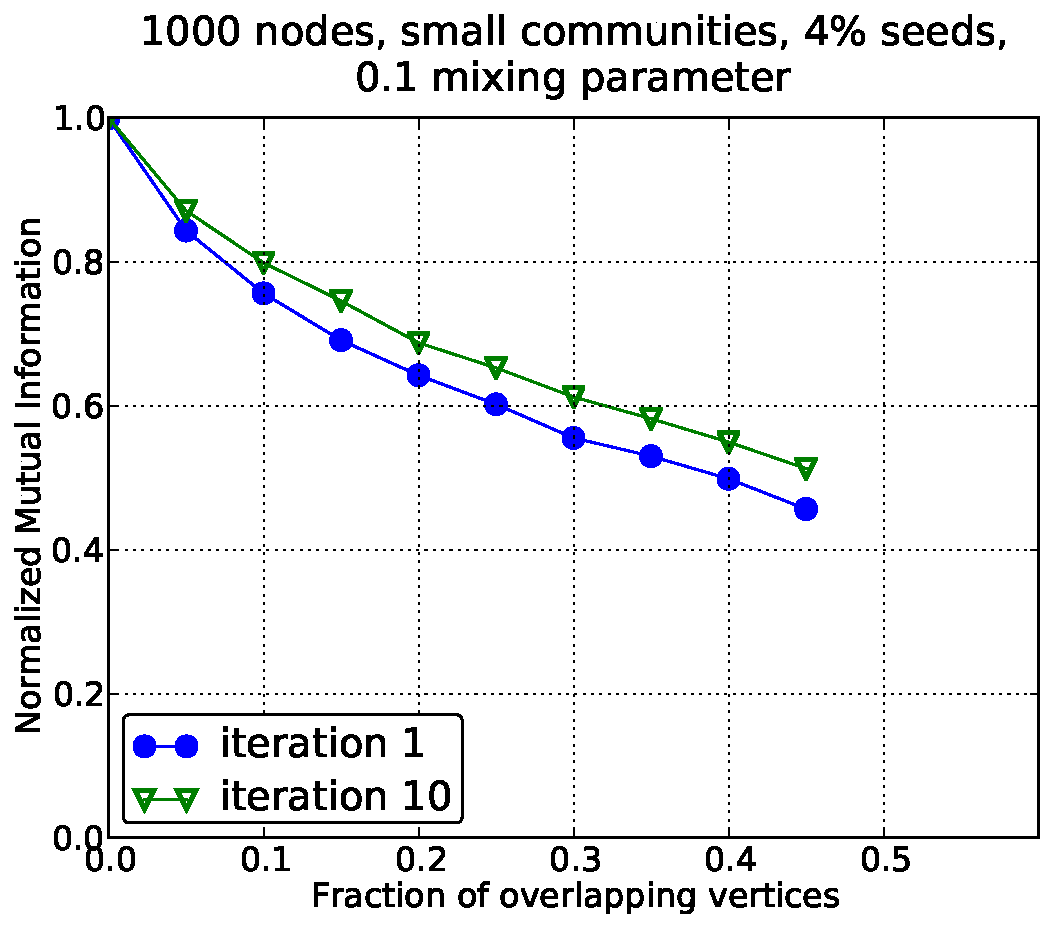
\includegraphics[width=\plotwidth]{plots/overlap_compare_a.pdf}
%    \end{subfigure}%
%    \begin{subfigure}{0.5\textwidth}
%    \centering
%    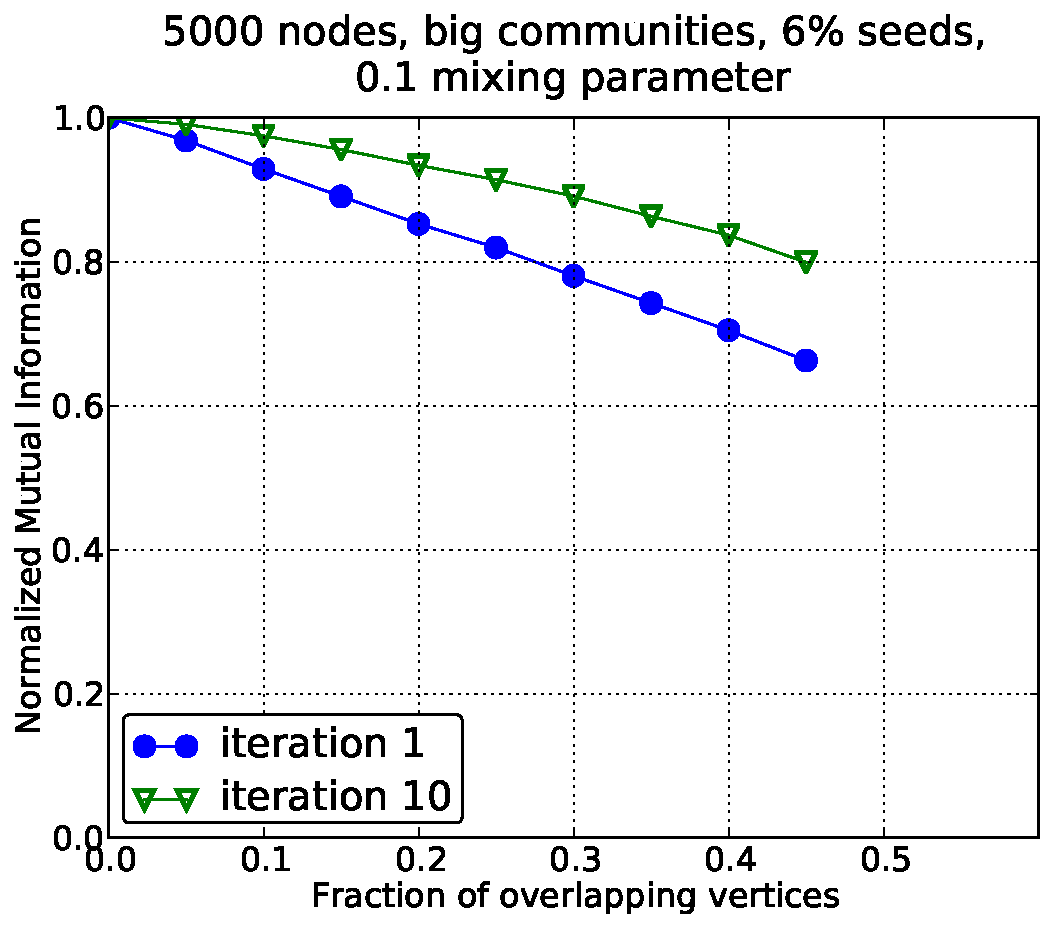
\includegraphics[width=\plotwidth]{plots/overlap_compare_b.pdf}
%    \end{subfigure}
%    \caption{Comparison between the iterative and non-iterative method for overlapping communities.}\label{fig:compare_iter_overlap}
%\end{figure}
%
\begin{figure}[h!]
    \centering
    \begin{subfigure}{0.5\textwidth}
    \centering
    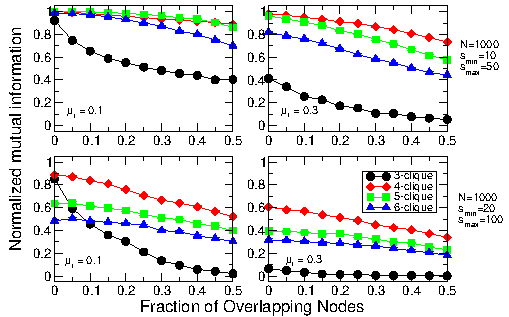
\includegraphics[width=\cfinderwidth]{lfrpaper/fig6.pdf}
    \end{subfigure}%
    \begin{subfigure}{0.5\textwidth}
    \centering
    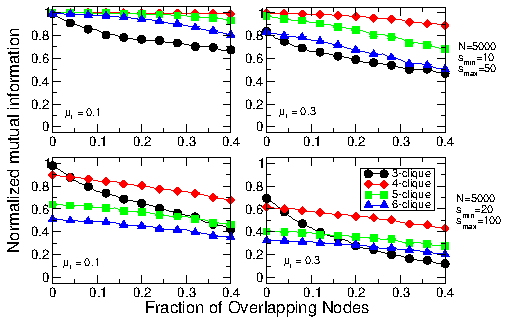
\includegraphics[width=\cfinderwidth]{lfrpaper/fig7.pdf}
    \end{subfigure}%
    \caption{
        Plots for CFinder on the LFR benchmark on graphs with 1000 and 5000 nodes 
		with overlapping communities. Reproduced from~\cite{LF09}.
    }\label{fig:CFinder_overlapping}
\end{figure}



\subsection{Overlapping communities}
Figures~\ref{fig:no_iter_overlap_1000N} and~\ref{fig:no_iter_overlap_5000N} 
show our results for the overlapping case. In the study of Lancichinetti and Fortunato~\cite{LF09}, 
only one algorithm (\emph{Cfinder}~\cite{PDFV05}) for overlapping communities was benchmarked 
(see Figure~\ref{fig:CFinder_overlapping}). 
The main difference with the non-overlapping case is that typically our algorithm needs a larger 
seed node percentage per community. This is not surprising since in the overlapping case, we would 
need seed nodes from the various overlaps as well as from the non-overlapping portions of communities 
to make a good-enough calculation of the affinities. 

For graphs of both 1000 and 5000 nodes, our algorithm performs better 
than Cfinder up to an overlapping fraction of $0.4$. We stress that Cfinder 
has an exponential worst-case running time and would be infeasible on larger graphs. 
%
Figures~\ref{fig:iter_overlap_1000N} and~\ref{fig:iter_overlap_5000N} show the 
plots for the iterative method (with 10 iterations). 
%A comparison of the non-iterative and iterative method is shown in 
%Figure~\ref{fig:compare_iter_overlap}. 
%Iteration yields an improvement in performance, as measured by the NMI, but it is 
%not as dramatic as in the non-overlapping case with the NMI increase being at most 
%$10\%$ at best. 
The percentage of seed nodes per community required in the 
iterative approach with a mixing factor of $0.3$ is around 8$\%$. 

\section{Concluding Remarks}

We wish to point out that while the running time of our algorithm is 
$O(k \cdot m \cdot \log n)$, we do not know of any commercial solvers 
for SDD systems that run in $O(m \cdot \log n)$ time. Since we use the Cholesky 
factorization method from the \CPP\ Eigen Library, it is unlikely that our 
implementation would be able to handle very large networks. Recall that 
in Cholesky factorization, the matrix of coefficients $\mat{A}$ is decomposed 
as $\mat{L} \mat{D} \trans{\mat{L}}$, where $\mat{L}$ is lower triangular 
and $\mat{D}$ is diagonal, all of which takes $n^3/3$ operations making it 
prohibitively expensive for large networks (see, for instance~\cite{GvL13}). 
This is not a serious disadvantage since we expect that in the near future 
we would have commercial SDD solvers implementing the Speilman-Teng algorithm. 
It would then be interesting to see the size range of real networks our algorithm 
can handle. 







\section{Experimental Results}
%width of the three types of plots
\newcommand{\appplotwidth}{\linewidth}
%\newcommand{\cfinderwidth}{0.96\linewidth}
%\newcommand{\otherplotswidth}{0.76\linewidth}

Here we give the complete results of our experiments, first for the non-overlapping case and then for the overlapping communities.

\subsection{Non-overlapping communities}
Figures~\ref{fig:no_iter_no_overlap} and \ref{fig:iter_no_overlap} %and~\ref{fig:compare_iter_no_overlap}
show the plots that we obtained for non-overlapping communities. Figure~\ref{fig:no_iter_no_overlap}
shows tests for the non-iterative method of our algorithm with 5, 10, 15, and 20$\%$ seed nodes per 
community. 

The first observation here is that anything less than 10$\%$ seed nodes per community 
do not give good results. With a seed node percentage of 10$\%$ or more and 
a mixing factor of at most~$0.4$ we achieve an NMI above $0.9$ and can compete with \textit{Infomap}, 
which was deemed to be one the best performing algorithms on the LFR benchmark~\cite{LF09}. 
Above a mixing factor of $0.4$, our algorithm has a worse performance than \textit{Infomap} 
which, curiously enough, achieves an NMI of around 1 till a mixing factor of around 
$0.6$ after which its performance drops steeply. The drop in the performance of our algorithm 
begins earlier but is not as steep. See Figure~\ref{fig:Infomap_etal} for the performance 
of Infomap and other algorithms that were studied in~\cite{LF09}. 

Figure~\ref{fig:iter_no_overlap} shows the results for the iterative approach of 
our algorithm in the non-overlapping case. When compared with the non-iterative approach, 
we found that even after ten iterations there is a significant improvement in 
performance. %(See Figure~\ref{fig:compare_iter_no_overlap}). 
As can be seen, typically with 6$\%$ seed nodes per community we obtain 
acceptable performance (an NMI value of over $0.9$ with the mixing factor 
of up to $0.5$).  


\begin{figure}[h!]
    \centering
    \begin{subfigure}{0.5\textwidth}
    \centering
    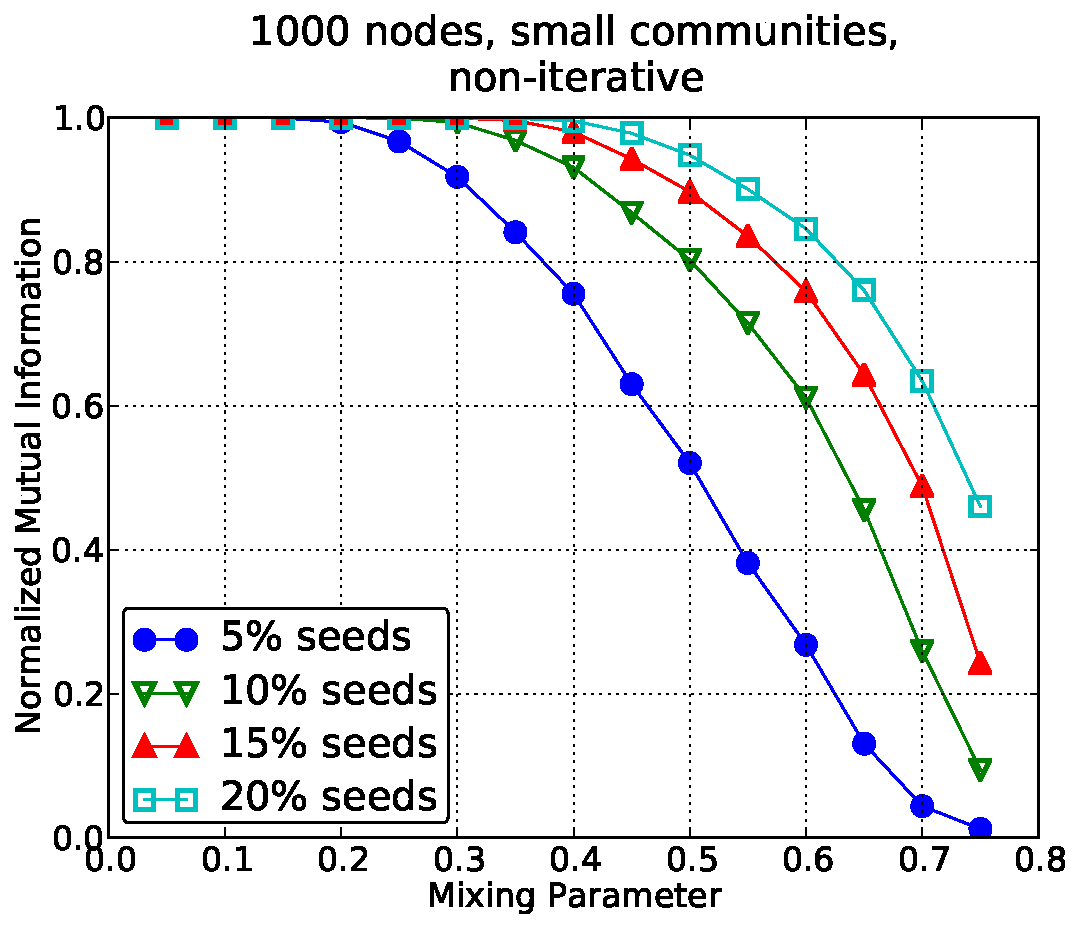
\includegraphics[width=\appplotwidth]{plots/nonoverlap_noniter_a.pdf}
    \end{subfigure}%
    \begin{subfigure}{0.5\textwidth}
    \centering
    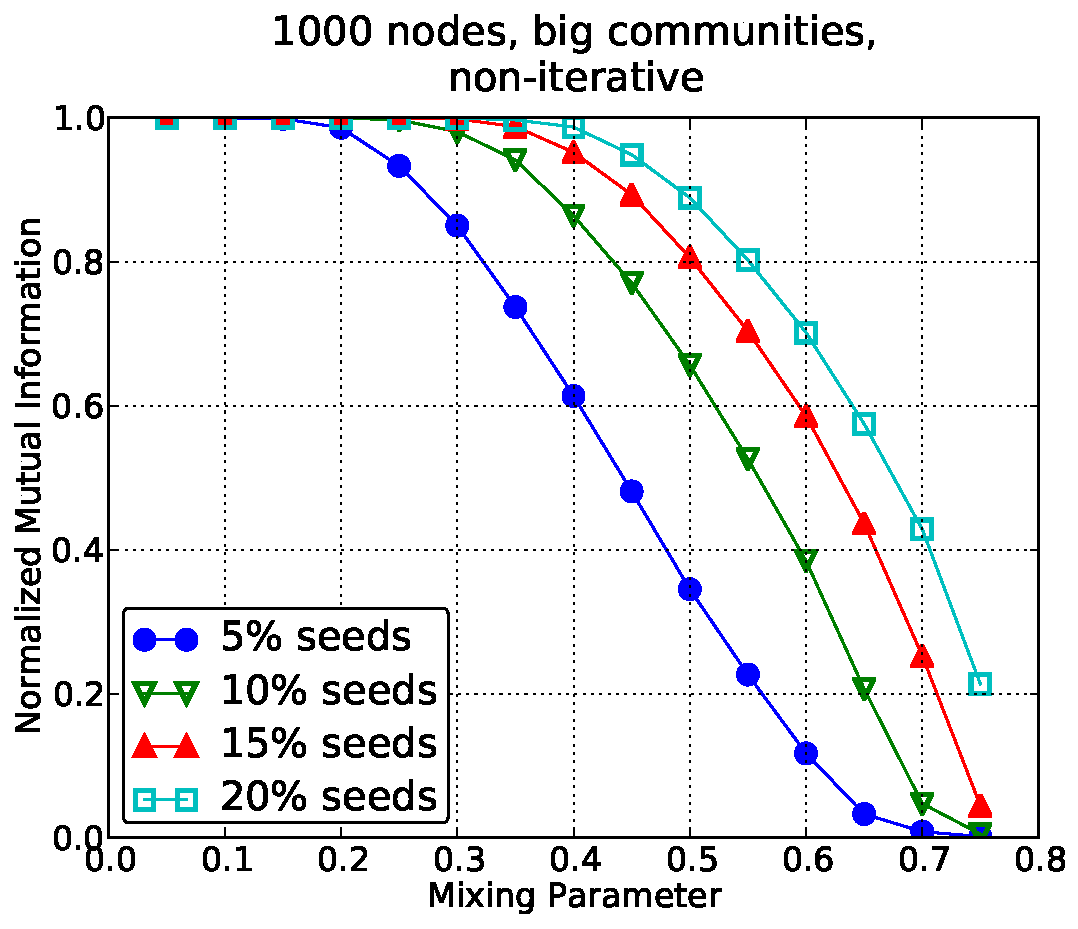
\includegraphics[width=\appplotwidth]{plots/nonoverlap_noniter_b.pdf}
    \end{subfigure}
    \begin{subfigure}{0.5\textwidth}
    \centering
    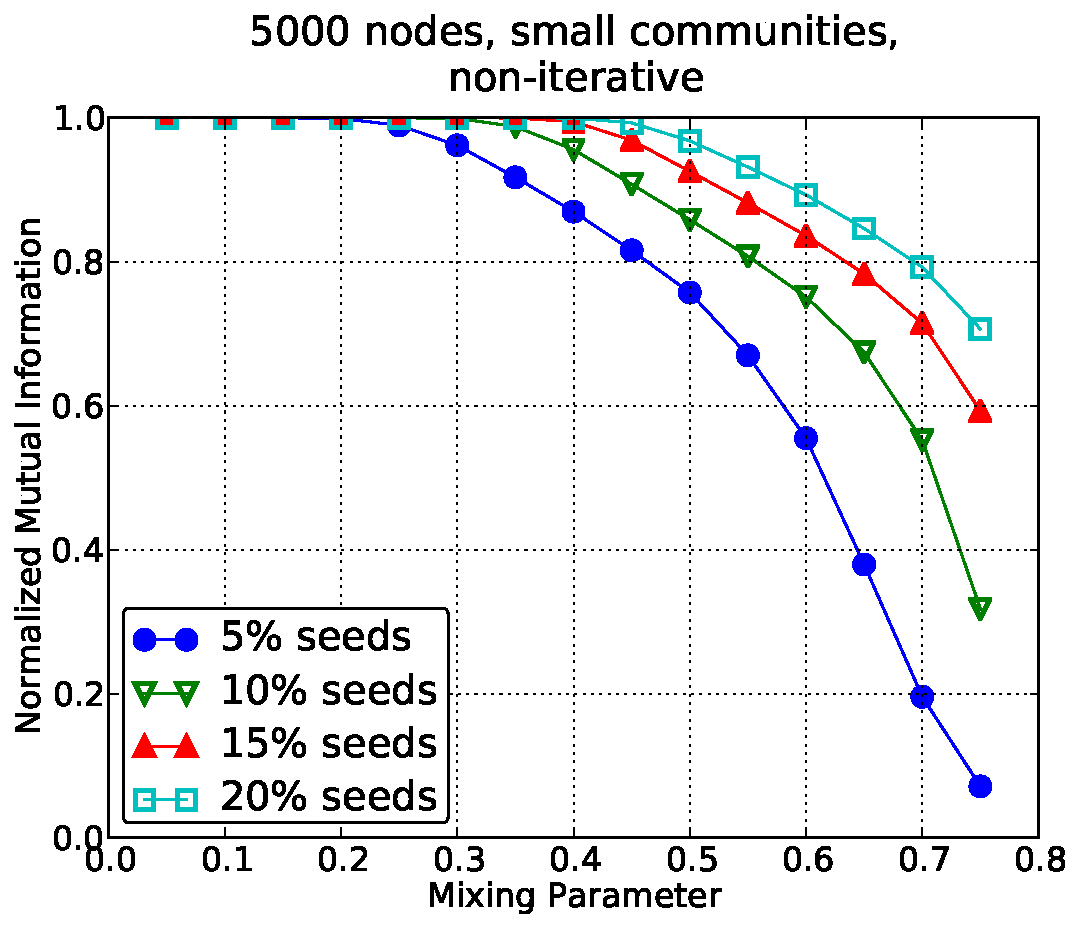
\includegraphics[width=\appplotwidth]{plots/nonoverlap_noniter_c.pdf}
    \end{subfigure}%
    \begin{subfigure}{0.5\textwidth}
    \centering
    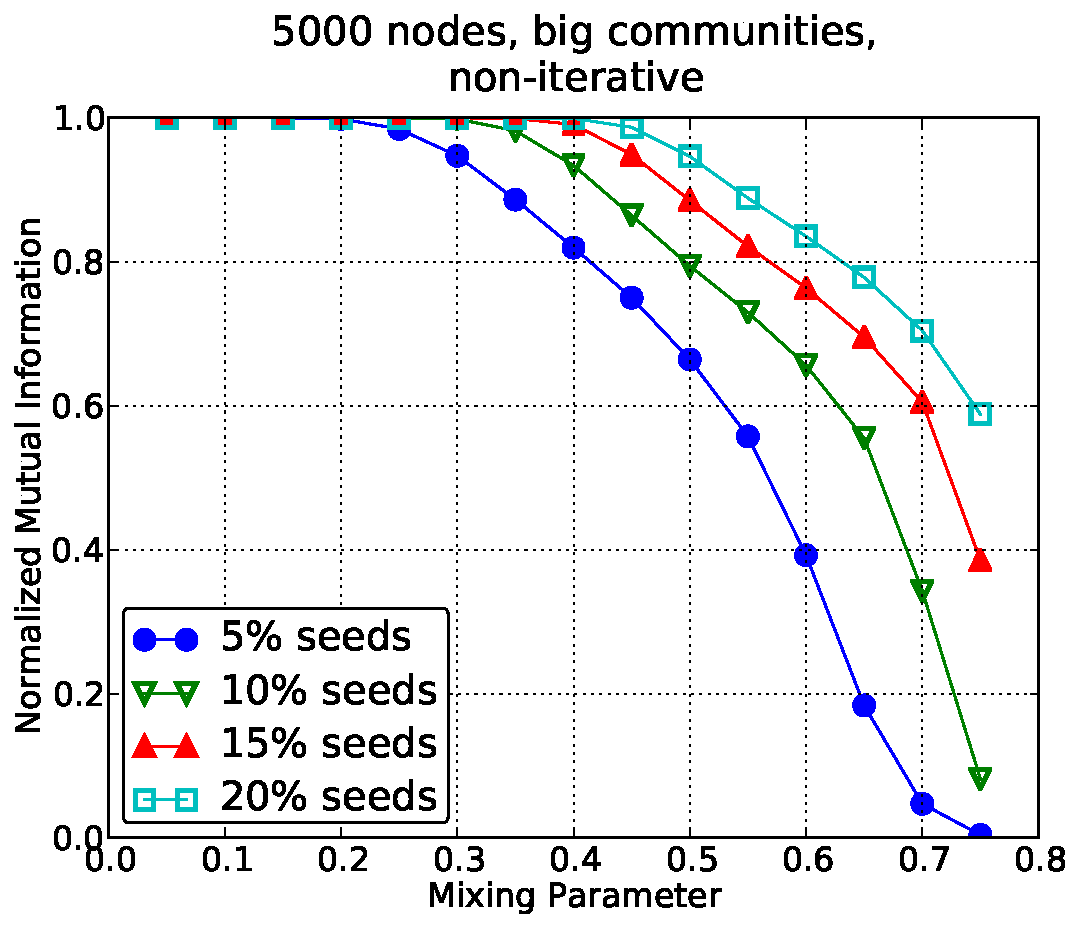
\includegraphics[width=\appplotwidth]{plots/nonoverlap_noniter_d.pdf}
    \end{subfigure}
    \caption{Non-iterative method for non-overlapping communities.}\label{fig:no_iter_no_overlap}
\end{figure}
%
\begin{figure}[h!]
    \centering
    \begin{subfigure}{0.5\textwidth}
    \centering
    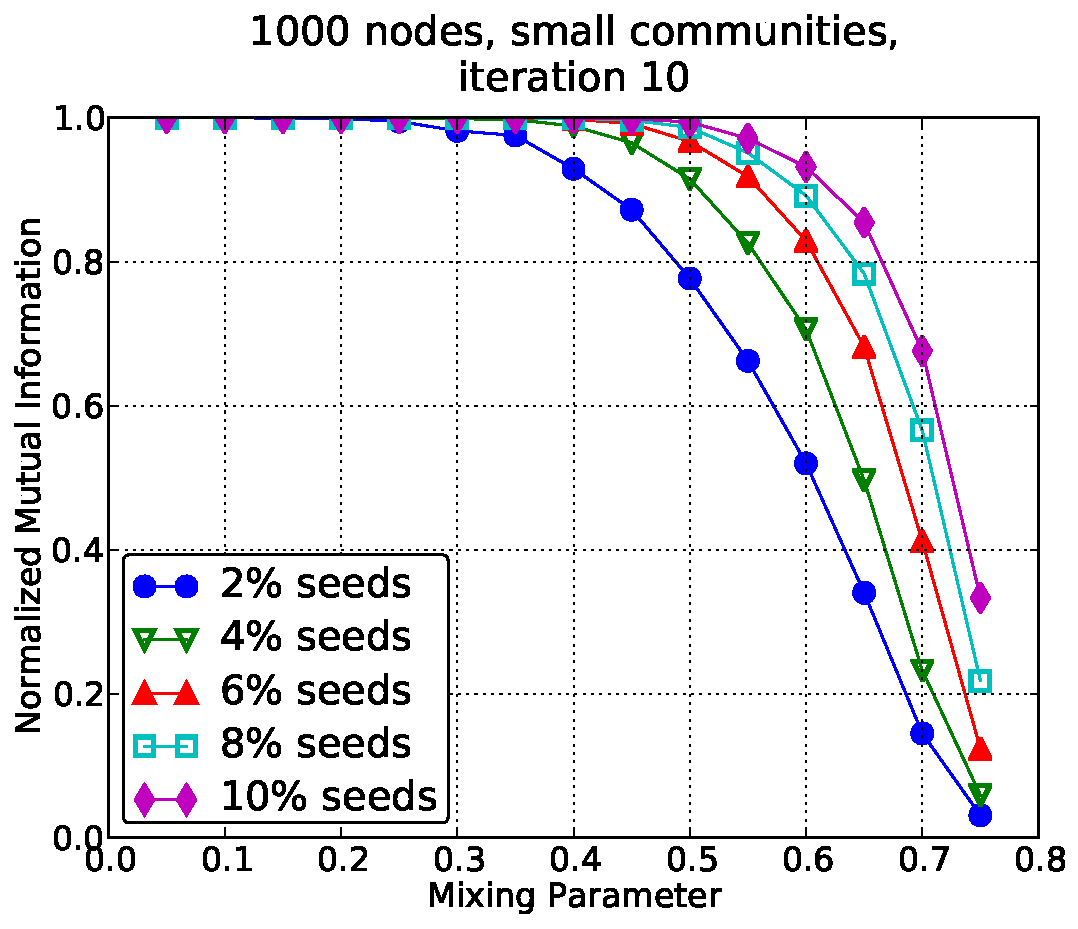
\includegraphics[width=\appplotwidth]{plots/nonoverlap_iter_a.pdf}
    \end{subfigure}%
    \begin{subfigure}{0.5\textwidth}
    \centering
    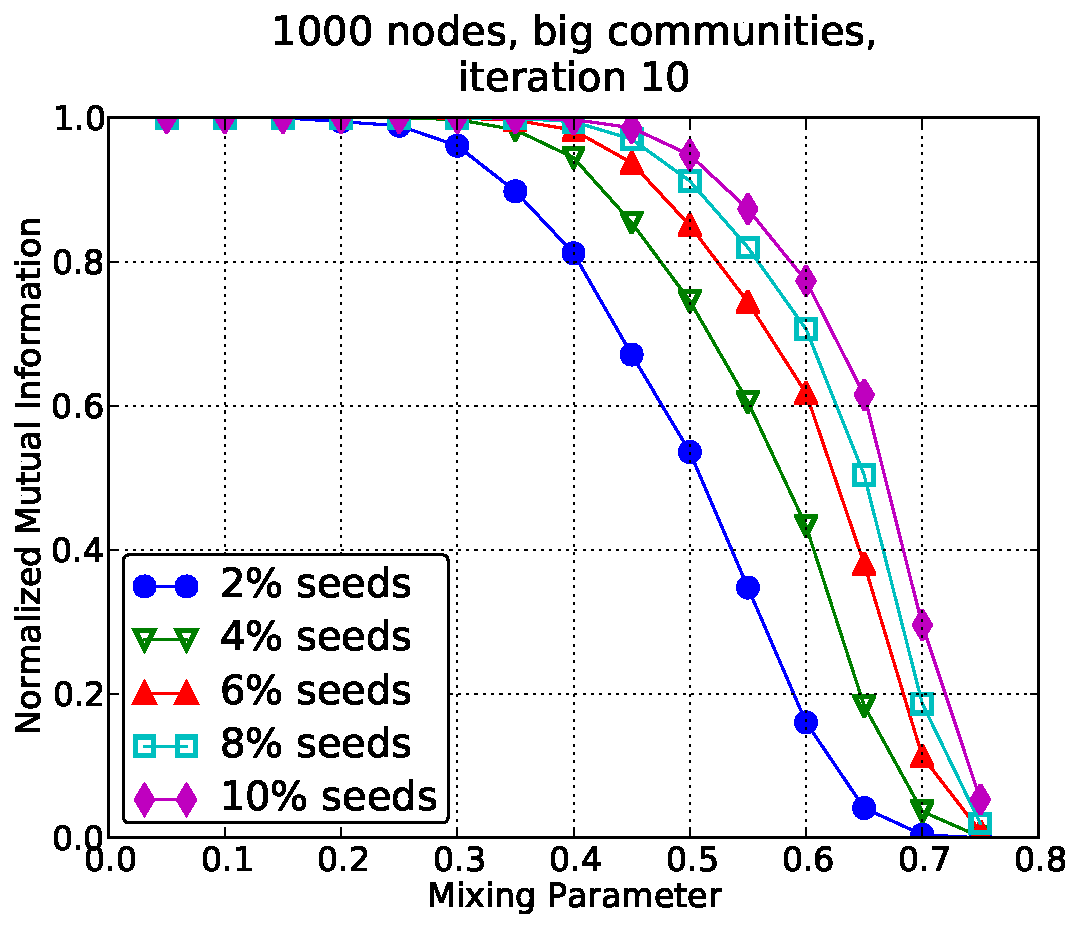
\includegraphics[width=\appplotwidth]{plots/nonoverlap_iter_b.pdf}
    \end{subfigure}
    \begin{subfigure}{0.5\textwidth}
    \centering
    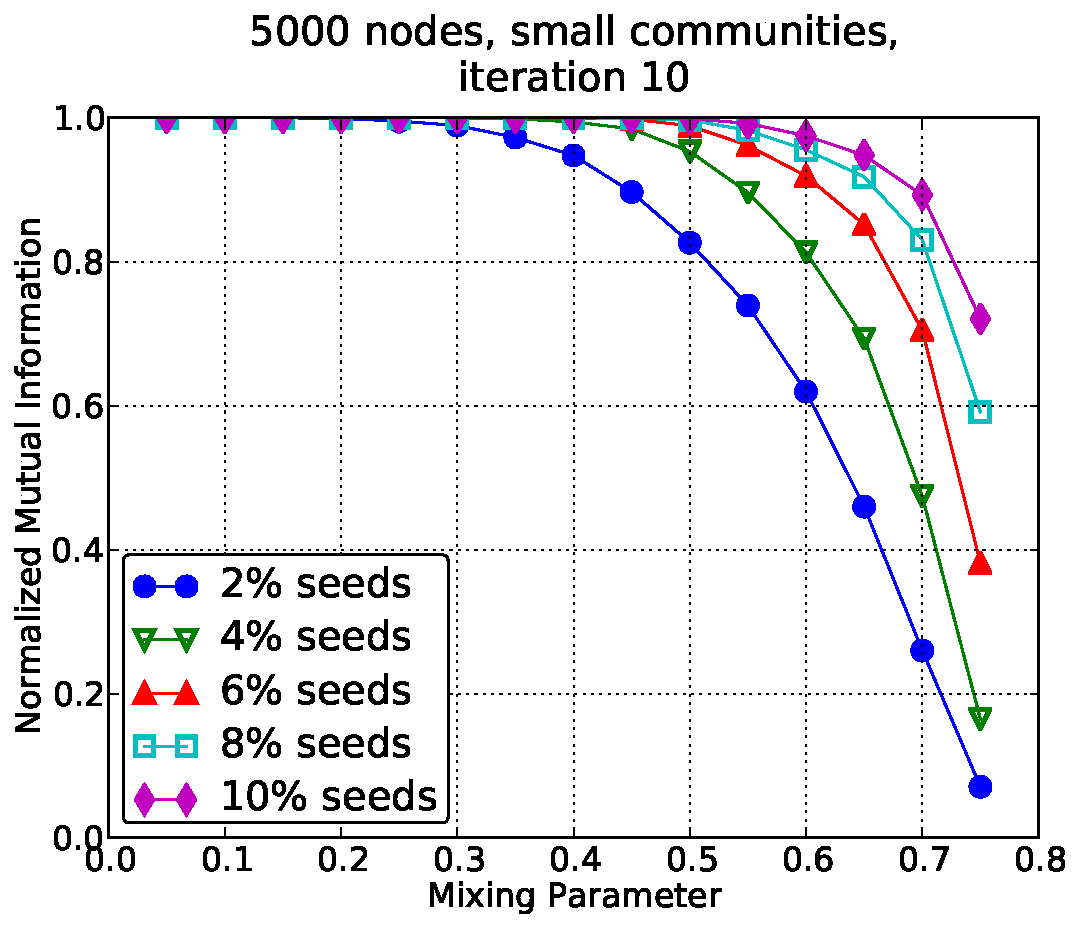
\includegraphics[width=\appplotwidth]{plots/nonoverlap_iter_c.pdf}
    \end{subfigure}%
    \begin{subfigure}{0.5\textwidth}
    \centering
    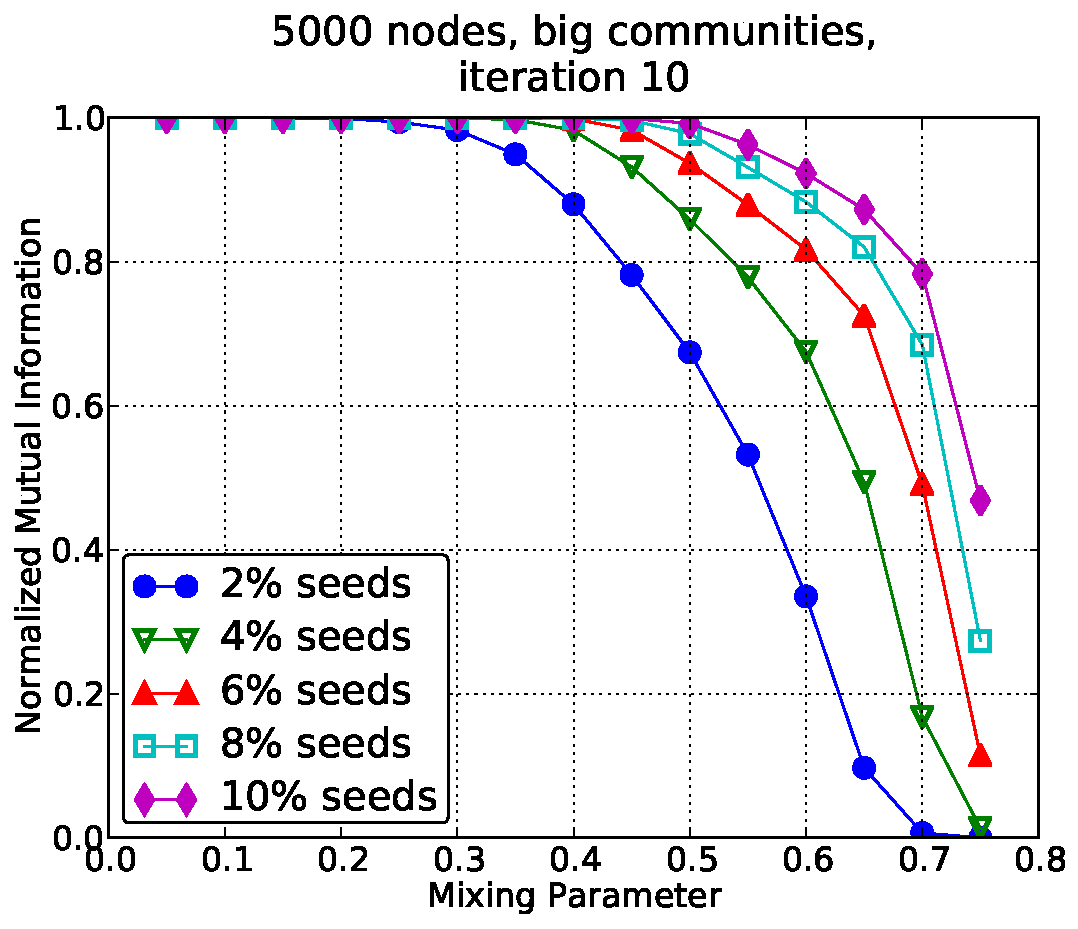
\includegraphics[width=\appplotwidth]{plots/nonoverlap_iter_d.pdf}
    \end{subfigure}
    \caption{Iterative method for non-overlapping communities.}\label{fig:iter_no_overlap}
\end{figure}
%

%\begin{figure}[h!]
%    \centering
%    \begin{subfigure}{0.5\textwidth}
%    \centering
%    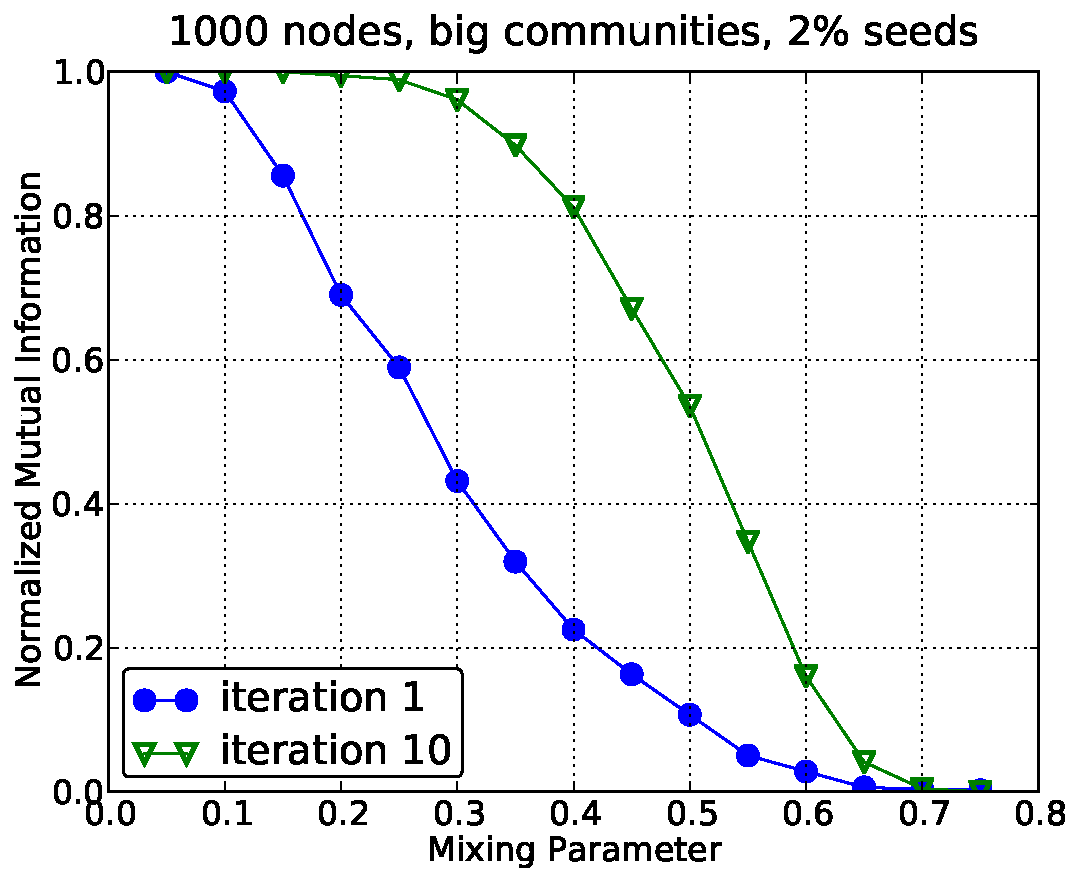
\includegraphics[width=\plotwidth]{plots/nonoverlap_compare_a.pdf}
%    \end{subfigure}%
%    \begin{subfigure}{0.5\textwidth}
%    \centering
%    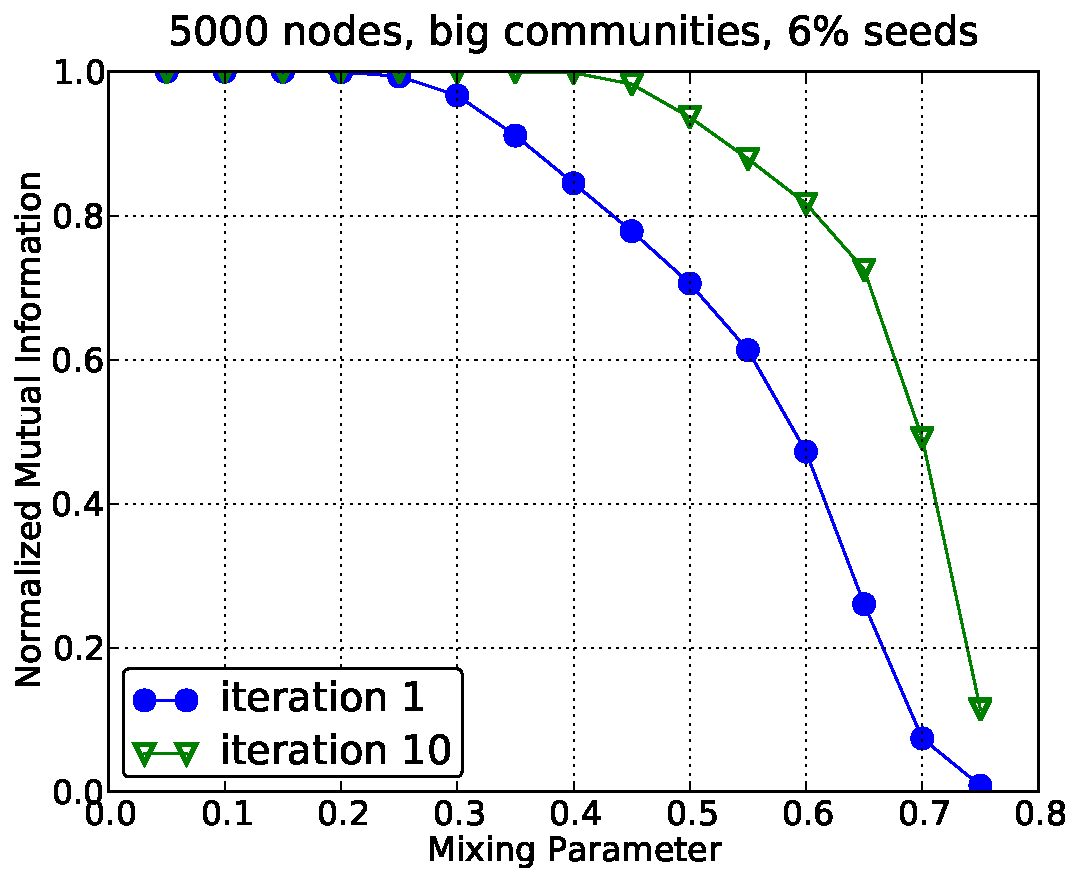
\includegraphics[width=\plotwidth]{plots/nonoverlap_compare_b.pdf}
%    \end{subfigure}
%    \caption{Comparison between the iterative and non-iterative method for 
%		non-overlapping communities.}\label{fig:compare_iter_no_overlap}
%\end{figure}

\begin{figure}[h!]
    \centering
    \begin{subfigure}{0.35\textwidth}
    \centering
    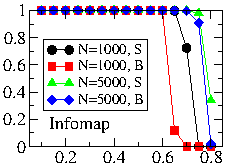
\includegraphics[width=\otherplotswidth]{lfrpaper/1_split_kropped.pdf}
    \end{subfigure}%
    \begin{subfigure}{0.35\textwidth}
    \centering
    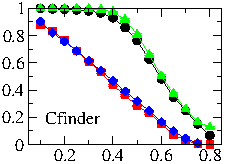
\includegraphics[width=\otherplotswidth]{lfrpaper/2_split_kropped.pdf}
    \end{subfigure}%
    \begin{subfigure}{0.35\textwidth}
    \centering
    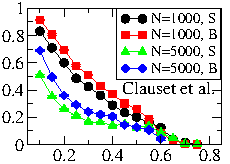
\includegraphics[width=\otherplotswidth]{lfrpaper/3_split_kropped.pdf}
    \end{subfigure}
    \begin{subfigure}{0.35\textwidth}
    \centering
    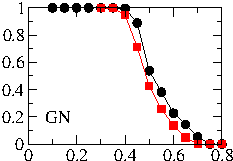
\includegraphics[width=\otherplotswidth]{lfrpaper/4_split_kropped.pdf}
    \end{subfigure}%
    \begin{subfigure}{0.35\textwidth}
    \centering
    \includegraphics[width=\otherplotswidth]{lfrpaper/5_split_kropped.pdf}
    \end{subfigure}%
    \begin{subfigure}{0.35\textwidth}
    \centering
    \includegraphics[width=\otherplotswidth]{lfrpaper/6_split_kropped.pdf}
    \end{subfigure}%
    \caption{
        Plots for Infomap, CFinder, the algorithm of Clauset \etal, Girvan-Newman (GN), Blondel \etal, 
        and the Pott's model approach by Ronhovde and Nussinov (RN) on the LFR benchmark for non-overlapping 
		communities. As usual, the NMI-value ($y$-axis) is plotted against the mixing factor ($x$-axis).
        Tests were performed on graphs with 1000 and 5000 nodes with big (B) and small (S) communities.
        Reproduced from~\cite{LF09}.
    }\label{fig:Infomap_etal}
\end{figure}

\begin{figure}[h!]
    \centering
    \begin{subfigure}{0.5\textwidth}
    \centering
    \includegraphics[width=\appplotwidth]{plots/overlap_noniter_1mu_a.pdf}
    \end{subfigure}%
    \begin{subfigure}{0.5\textwidth}
    \centering
    \includegraphics[width=\appplotwidth]{plots/overlap_noniter_3mu_a.pdf}
    \end{subfigure}
    \begin{subfigure}{0.5\textwidth}
    \centering
    \includegraphics[width=\appplotwidth]{plots/overlap_noniter_1mu_b.pdf}
    \end{subfigure}%
    \begin{subfigure}{0.5\textwidth}
    \centering
    \includegraphics[width=\appplotwidth]{plots/overlap_noniter_3mu_b.pdf}
    \end{subfigure}
    \caption{Non-iterative method for overlapping communities on 1000 nodes.}\label{fig:no_iter_overlap_1000N}
\end{figure}
%
\begin{figure}[h!]
    \centering
    \begin{subfigure}{0.5\textwidth}
    \centering
    \includegraphics[width=\appplotwidth]{plots/overlap_noniter_1mu_c.pdf}
    \end{subfigure}%
    \begin{subfigure}{0.5\textwidth}
    \centering
    \includegraphics[width=\appplotwidth]{plots/overlap_noniter_3mu_c.pdf}
    \end{subfigure}
    \begin{subfigure}{0.5\textwidth}
    \centering
    \includegraphics[width=\appplotwidth]{plots/overlap_noniter_1mu_d.pdf}
    \end{subfigure}%
    \begin{subfigure}{0.5\textwidth}
    \centering
    \includegraphics[width=\appplotwidth]{plots/overlap_noniter_3mu_d.pdf}
    \end{subfigure}
    \caption{Non-iterative method for overlapping communities on 5000 nodes.}\label{fig:no_iter_overlap_5000N}
\end{figure}
%
\begin{figure}[h!]
    \centering
    \begin{subfigure}{0.5\textwidth}
    \centering
    \includegraphics[width=\appplotwidth]{plots/overlap_iter_1mu_a.pdf}
    \end{subfigure}%
    \begin{subfigure}{0.5\textwidth}
    \centering
    \includegraphics[width=\appplotwidth]{plots/overlap_iter_1mu_b.pdf}
    \end{subfigure}
    \begin{subfigure}{0.5\textwidth}
    \centering
    \includegraphics[width=\appplotwidth]{plots/overlap_iter_3mu_a.pdf}
    \end{subfigure}%
    \begin{subfigure}{0.5\textwidth}
    \centering
    \includegraphics[width=\appplotwidth]{plots/overlap_iter_3mu_b.pdf}
    \end{subfigure}
    \caption{Iterative method for overlapping communities on 1000 nodes.}\label{fig:iter_overlap_1000N}
\end{figure}
%
\begin{figure}[h!]
    \centering
    \begin{subfigure}{0.5\textwidth}
    \centering
    \includegraphics[width=\appplotwidth]{plots/overlap_iter_1mu_c.pdf}
    \end{subfigure}%
    \begin{subfigure}{0.5\textwidth}
    \centering
    \includegraphics[width=\appplotwidth]{plots/overlap_iter_1mu_d.pdf}
    \end{subfigure}
    \begin{subfigure}{0.5\textwidth}
    \centering
    \includegraphics[width=\appplotwidth]{plots/overlap_iter_3mu_c.pdf}
    \end{subfigure}%
    \begin{subfigure}{0.5\textwidth}
    \centering
    \includegraphics[width=\appplotwidth]{plots/overlap_iter_3mu_d.pdf}
    \end{subfigure}
    \caption{Iterative method for overlapping communities on 5000 nodes.}\label{fig:iter_overlap_5000N}
\end{figure}
%
%\begin{figure}[h!]
%    \centering
%    \begin{subfigure}{0.5\textwidth}
%    \centering
%    \includegraphics[width=\plotwidth]{plots/overlap_compare_a.pdf}
%    \end{subfigure}%
%    \begin{subfigure}{0.5\textwidth}
%    \centering
%    \includegraphics[width=\plotwidth]{plots/overlap_compare_b.pdf}
%    \end{subfigure}
%    \caption{Comparison between the iterative and non-iterative method for overlapping communities.}\label{fig:compare_iter_overlap}
%\end{figure}
%
\begin{figure}[h!]
    \centering
    \begin{subfigure}{0.5\textwidth}
    \centering
    \includegraphics[width=\cfinderwidth]{lfrpaper/fig6.pdf}
    \end{subfigure}%
    \begin{subfigure}{0.5\textwidth}
    \centering
    \includegraphics[width=\cfinderwidth]{lfrpaper/fig7.pdf}
    \end{subfigure}%
    \caption{
        Plots for CFinder on the LFR benchmark on graphs with 1000 and 5000 nodes 
		with overlapping communities. Reproduced from~\cite{LF09}.
    }\label{fig:CFinder_overlapping}
\end{figure}



\subsection{Overlapping communities}
Figures~\ref{fig:no_iter_overlap_1000N} and~\ref{fig:no_iter_overlap_5000N} 
show our results for the overlapping case. In the study of Lancichinetti and Fortunato~\cite{LF09}, 
only one algorithm (\emph{Cfinder}~\cite{PDFV05}) for overlapping communities was benchmarked 
(see Figure~\ref{fig:CFinder_overlapping}). 
The main difference with the non-overlapping case is that typically our algorithm needs a larger 
seed node percentage per community. This is not surprising since in the overlapping case, we would 
need seed nodes from the various overlaps as well as from the non-overlapping portions of communities 
to make a good-enough calculation of the affinities. 

For graphs of both 1000 and 5000 nodes, our algorithm performs better 
than Cfinder up to an overlapping fraction of $0.4$. We stress that Cfinder 
has an exponential worst-case running time and would be infeasible on larger graphs. 
%
Figures~\ref{fig:iter_overlap_1000N} and~\ref{fig:iter_overlap_5000N} show the 
plots for the iterative method (with 10 iterations). 
%A comparison of the non-iterative and iterative method is shown in 
%Figure~\ref{fig:compare_iter_overlap}. 
%Iteration yields an improvement in performance, as measured by the NMI, but it is 
%not as dramatic as in the non-overlapping case with the NMI increase being at most 
%$10\%$ at best. 
The percentage of seed nodes per community required in the 
iterative approach with a mixing factor of $0.3$ is around 8$\%$. 





